\documentclass[conference]{IEEEtran}
\IEEEoverridecommandlockouts

\usepackage{cite}
\usepackage{amsmath,amssymb}
\usepackage{graphicx}
\usepackage{booktabs}
\usepackage{multirow}
\usepackage{array}
\usepackage{url}
\usepackage{xcolor}
\usepackage{tikz}
\usetikzlibrary{positioning,arrows.meta,fit}
\usepackage{pgfplots}
\pgfplotsset{compat=1.17}

\newcommand{\pmse}[2]{#1\,$\pm$\,#2}
\newcommand{\todo}[1]{\textcolor{red}{[TODO: #1]}}

\begin{document}

\title{Multimodal Crisis Diagnosis: A Disaster-Tweet\\Triage Pipeline on CrisisMMD}

\author{
\IEEEauthorblockN{Anurag V Rao}
\IEEEauthorblockA{\textit{Dept. of Information Technology}\\
\textit{National Institute of Technology}\\
Karnataka, Surathkal, India\\
anuragvrao.241it011@nitk.edu.in}
\and
\IEEEauthorblockN{Chhitanshu Shekhar}
\IEEEauthorblockA{\textit{Dept. of Information Technology}\\
\textit{National Institute of Technology}\\
Karnataka, Surathkal, India\\
chhitanshushekhar.241ai012@nitk.edu.in}
\and
\IEEEauthorblockN{Dr. Sowmya Kamath S}
\IEEEauthorblockA{\textit{Dept. of Information Technology}\\
\textit{National Institute of Technology}\\
Karnataka, Surathkal, India\\
sowmyakamath@nitk.edu.in}
}

\maketitle

% =====================================================================
\begin{abstract}
Social-media posts during disasters pair text with images that may agree, complement or contradict each other. We present a three-task triage pipeline on CrisisMMD v2.0 that flags informativeness from the tweet text with a fine-tuned BERTweet, assigns one of eight humanitarian categories with a cross-attention fusion of a fine-tuned DistilBERT and frozen CLIP image features, and grades damage severity with a logistic-regression probe whose prediction is accompanied by the five most similar past cases. When the probe and the retrieved cases disagree, the prediction is flagged for human review. On the official test splits the pipeline reaches, as means over three seeds, a weighted F1 of 0.838 and a macro-F1 of 0.797 on Task~1, and macro-F1 of 0.598 and 0.615 on Tasks~2 and~3. We compare it with our earlier version through a ladder of single changes scored on a common leakage-free test set, with three seeds and paired bootstrap intervals. Restoring two earthquake events that a path-handling defect had removed gives the only established humanitarian gain (+0.095 macro-F1), and removing test images from the retrieval index shows that the earlier damage score of 0.688 was 0.378 in practice. Ablations with selection rules fixed in advance show that the image carries the humanitarian task, that text helps only where the text and image labels agree, and that a larger CLIP encoder is the only design choice resolvable on development data. At our guide's request we also compared the candidate models for Tasks~1 and~2 under rules fixed in advance: a fine-tuned BERTweet replaced TF-IDF with logistic regression for Task~1 (development weighted-F1 gain +0.0195, 95\% interval [+0.0049, +0.0340]), whereas the guide's early-fusion model (BERTweet with a frozen ResNet50) was not better than our Task~2 model, and in both tasks fusion helps only where the text and image labels agree. Probe--retrieval agreement separates reliable damage predictions (accuracy 0.812) from those needing review (0.446).
\end{abstract}

\begin{IEEEkeywords}
crisis informatics, multimodal learning, disaster response, CLIP, retrieval, ablation, data leakage, class imbalance, calibration
\end{IEEEkeywords}

% =====================================================================
\section{Introduction}

In the hours after a natural disaster, platforms such as Twitter carry large volumes of posts from eyewitnesses, affected people, journalists and volunteers, many with attached images. For humanitarian organisations this content is valuable but hard to use: actionable reports are buried among reposts, opinions and messages that are emotionally expressive but operationally irrelevant~\cite{imran2015}. Images frequently carry information that the text does not, and the two modalities can disagree, so text-only systems miss part of the picture~\cite{alam2018,ofli2020}.

Responders cannot read every post, so triage needs automatic answers to three questions: is the post informative, which humanitarian need does it express, and how severe is the damage it shows. We address these on the CrisisMMD v2.0 benchmark~\cite{alam2018} as Task~1 (informativeness), Task~2 (eight humanitarian categories) and Task~3 (three damage-severity levels).

An initial version of the pipeline was developed in the previous phase of this project. In this phase we redesigned it and, at our guide's request, compared the two versions rigorously: every change between them is isolated and evaluated on the same test set, with three training seeds and bootstrap confidence intervals. Leakage between training and test data is a well-documented source of over-optimistic results in applied machine learning~\cite{kapoor2023}, so the comparison is built on explicit checks of split integrity. We then tested the remaining design choices under selection rules committed before the runs.

The contributions of this project are:
\begin{itemize}
\item a three-task triage pipeline in which damage severity is predicted by a trained probe and explained by retrieved past cases, with probe--retrieval agreement used to flag predictions for human review;
\item a reproducible comparison with our earlier version: a ladder of single changes on a common leakage-free test set, three seeds, paired bootstrap intervals, and an automated check of every reported number against stored results;
\item component, robustness, class-imbalance and architecture ablations showing that the image carries the humanitarian task, that fusion helps only where the two labels agree (in both Task~1 and Task~2), and that a held-out earthquake mainly costs the rare \emph{injured or dead people} class;
\item a comparison of the candidate models of the guide's lists for Tasks~1 and~2 (classical, recurrent, BERTweet, image heads and three fusion designs) under rules committed before the runs, with a unified agreed/disagreed analysis, a fusion-gain analysis and a rule-based error analysis (Section~\ref{sec:explore});
\item an interactive triage tool that shows all three predictions, with temperature-calibrated confidence for all three tasks.
\end{itemize}

% =====================================================================
\section{Background and Related Work}

\subsection{CrisisMMD}
CrisisMMD~\cite{alam2018} contains tweets and their attached images collected during seven natural disasters of 2017: Hurricanes Harvey, Irma and Maria, the California wildfires, the Mexico earthquake, the Iraq--Iran earthquake and the Sri Lanka floods. Text and images were annotated separately for informativeness and humanitarian category, and images were additionally annotated for damage severity. Because the two modalities were labelled independently, a text and its image can carry different labels for the same task~\cite{ofli2020}.

\subsection{Multimodal Crisis Classification}
Ofli et al.~\cite{ofli2020} trained text CNNs, image CNNs and a multimodal fusion network on CrisisMMD and reported that fusion improves over either modality. Their experiments use the subset on which the text and image labels agree and merge several humanitarian classes into five. Our evaluation uses the full official splits with all eight humanitarian classes, so the settings differ (Section~\ref{sec:results}).

\subsection{Foundation Models and Retrieval}
CLIP~\cite{radford2021} learns aligned image and text embeddings from web-scale image--caption pairs, which makes its image features strong general-purpose descriptors. DistilBERT~\cite{sanh2019} is a compact transformer for fine-tuned text classification, and Sentence-BERT~\cite{reimers2019} with MiniLM~\cite{wang2020} or MPNet~\cite{song2020} backbones produces sentence embeddings suitable for similarity search. We also compare DINOv2~\cite{oquab2024} and ResNet-50~\cite{he2016} as image backbones. Our fusion uses multi-head cross-attention~\cite{vaswani2017}, and exact nearest-neighbour search is provided by FAISS~\cite{johnson2021}. Retrieved neighbours give an example-based explanation of a prediction, which helps a responder judge whether to trust it. For text we additionally compare BERTweet~\cite{nguyen2020}, a RoBERTa~\cite{liu2019} model pre-trained on English tweets, with classical baselines (naive Bayes, random forests~\cite{breiman2001} and linear SVMs as implemented in scikit-learn~\cite{pedregosa2011}) and a bidirectional LSTM~\cite{hochreiter1997,schuster1997} over GloVe vectors~\cite{pennington2014}.

\subsection{Class Imbalance, Calibration and Uncertainty}
For class imbalance we compare inverse-frequency weighting with class-balanced weights based on the effective number of samples~\cite{cui2019}, focal loss~\cite{lin2017} and logit adjustment~\cite{menon2021}. Modern neural classifiers are often over-confident; temperature scaling fitted on held-out data is a simple correction that does not change the predicted class~\cite{guo2017}. We report percentile bootstrap intervals~\cite{efron1993} for every comparison we call established.

% =====================================================================
\section{Dataset, Tasks and Split Integrity}

\subsection{Tasks}
\textbf{Task~1} labels a tweet as \emph{informative} or \emph{not informative} from its text. \textbf{Task~2} assigns one of eight humanitarian categories, scored against the image's annotation. \textbf{Task~3} grades the damage shown in the image as \emph{severe}, \emph{mild} or \emph{little or no damage}. Because Task~1 and Task~2 use different label sources, they can legitimately disagree on one tweet, and the system shows both when they do.

\subsection{Splits and Class Distribution}
We use the official \texttt{datasplit\_all} splits. Tasks~1 and~2 have 13,608 training, 2,237 development and 2,237 test pairs; Task~3 has 2,468, 529 and 529 (Table~\ref{tab:classes}). Imbalance is severe for Task~2: the largest-to-smallest training ratio is 729.4:1, against 2.4:1 for Task~1 and 4.6:1 for Task~3. \emph{Injured or dead people} has 10 test rows and \emph{missing or found people} only 3.

\begin{table}[t]
\centering
\caption{Class distribution of the official splits (rows per class).}
\label{tab:classes}
\footnotesize
\setlength{\tabcolsep}{4pt}
\begin{tabular}{llrrr}
\toprule
Task & Class & Train & Dev & Test \\
\midrule
\multirow{2}{*}{T1} & Informative & 9,638 & 1,612 & 1,612 \\
 & Not informative & 3,970 & 625 & 625 \\
\midrule
\multirow{8}{*}{T2} & Not humanitarian & 6,565 & 1,088 & 1,055 \\
 & Infrastructure and utility damage & 2,761 & 405 & 458 \\
 & Other relevant information & 1,860 & 338 & 331 \\
 & Rescue, volunteering or donation & 1,694 & 281 & 256 \\
 & Affected individuals & 397 & 77 & 88 \\
 & Vehicle damage & 230 & 38 & 36 \\
 & Injured or dead people & 92 & 8 & 10 \\
 & Missing or found people & 9 & 2 & 3 \\
\midrule
\multirow{3}{*}{T3} & Severe damage & 1,548 & 332 & 332 \\
 & Mild damage & 587 & 126 & 126 \\
 & Little or no damage & 333 & 71 & 71 \\
\bottomrule
\end{tabular}
\end{table}

\subsection{Tweet-Level Integrity}
\label{sec:data_integrity}
The official damage-severity splits separate images, not tweets. As a result, 62 test tweets (67 rows) have another image of the same tweet in the training split, and 16 tweets are shared between development and test. Because Task~3 retrieves training examples, such siblings would let a test query match its own tweet. The dataset authors avoid this by assigning all multi-image tweets to training~\cite{ofli2020}; we apply the same principle and exclude from the Task~3 index the 107 training rows that share a tweet with the test set, leaving 2,361 index rows. The informativeness and humanitarian splits are tweet-disjoint within each task, but not across tasks: 1,603 of the 2,237 Task~1 test rows are in the Task~2 training split (305 in its development split, 329 in its test split), and 328 are in the Task~3 index. A model for one task must therefore never use weights, logits or heads trained on another task's data. This is enforced by provenance fields (task, label column, hash of the training split, initialisation) stored with every run and checked by every script that consumes saved runs, and a retroactive audit found no violation. All of these properties are asserted in the code, as is the resolution of every image path in every split.

\subsection{Duplicate Images Across Tweets}
Tweet-level filtering cannot catch an identical image posted by a different tweet. Hashing all image files found 181 groups of byte-identical files, 175 of which span different tweet ids. Nine of the 529 Task~3 test images have an identical file in the index, three of them with a different severity label, and 68 of the 2,237 Task~2 test images have one in the training or development data. Counting near-duplicates as well (CLIP cosine similarity $\geq 0.98$), 24 Task~3 and 142 Task~2 test rows are flagged. Re-scoring the headline models without the flagged rows changes macro-F1 by at most 0.005 (Task~3 hybrid 0.615 to 0.619; Task~2 $-0.002$), so the duplicates do not inflate the reported results. \textbf{Task~1 split.} The same checks on the Task~1 split (test rows against its training rows) find 1 exact and 1 further near-duplicate test tweets (normalised text, TF-IDF cosine $\geq 0.9$) and 57 test images with a byte-identical file in the training split (0 with the same tweet id), 142 flagged in total with CLIP B/32 cosine $\geq 0.98$. Re-scoring without the flagged rows changes BERTweet's weighted F1 by +0.0001 (text duplicates removed) and by $-$0.0047 (image duplicates removed), and no image head or fusion model by more than 0.0051 in weighted F1 or 0.0034 in macro-F1.

% =====================================================================
\section{Methodology}

\begin{figure*}[t]
\centering
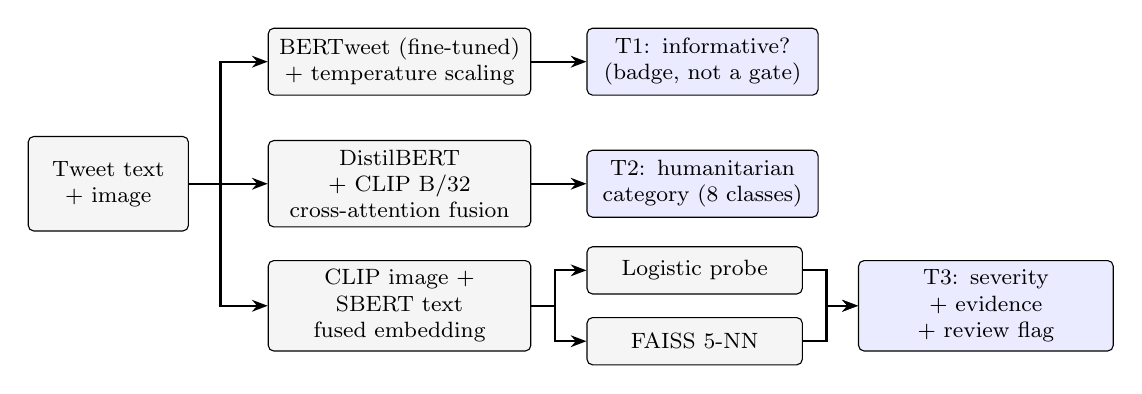
\begin{tikzpicture}[
  font=\footnotesize,
  box/.style={draw, rounded corners=2pt, fill=gray!8, align=center, minimum height=0.85cm, text width=3.1cm},
  outb/.style={draw, rounded corners=2pt, fill=blue!8, align=center, minimum height=0.85cm, text width=2.7cm},
  arr/.style={-{Stealth[length=2mm]}, thick},
  node distance=0.45cm and 0.7cm]
\node[box, text width=1.8cm, minimum height=1.2cm] (in) {Tweet text\\+ image};
\node[box, right=1.0cm of in, yshift=1.55cm] (t1) {BERTweet (fine-tuned)\\+ temperature scaling};
\node[box, right=1.0cm of in] (t2) {DistilBERT + CLIP B/32\\cross-attention fusion};
\node[box, right=1.0cm of in, yshift=-1.55cm] (t3a) {CLIP image + SBERT text\\fused embedding};
\node[outb, right=of t1] (o1) {T1: informative?\\(badge, not a gate)};
\node[outb, right=of t2] (o2) {T2: humanitarian\\category (8 classes)};
\node[box, right=of t3a, text width=2.5cm, yshift=0.45cm, minimum height=0.6cm] (p) {Logistic probe};
\node[box, right=of t3a, text width=2.5cm, yshift=-0.45cm, minimum height=0.6cm] (k) {FAISS 5-NN};
\node[outb, right=of p, yshift=-0.45cm, text width=3.0cm] (o3) {T3: severity + evidence\\+ review flag};
\draw[arr] (in.east) -- ++(0.4,0) |- (t1.west);
\draw[arr] (in.east) -- (t2.west);
\draw[arr] (in.east) -- ++(0.4,0) |- (t3a.west);
\draw[arr] (t1) -- (o1);
\draw[arr] (t2) -- (o2);
\draw[arr] (t3a.east) -- ++(0.3,0) |- (p.west);
\draw[arr] (t3a.east) -- ++(0.3,0) |- (k.west);
\draw[arr] (p.east) -- ++(0.3,0) |- (o3.west);
\draw[arr] (k.east) -- ++(0.3,0) |- (o3.west);
\end{tikzpicture}
\caption{Three-stage triage pipeline over one tweet. Task~1 is a fine-tuned BERTweet with a development-fitted temperature. All three tasks run on every request. Task~3 predicts with a trained probe; the five retrieved neighbours serve as evidence, and their agreement with the probe sets the confidence level.}
\label{fig:pipeline}
\end{figure*}

Fig.~\ref{fig:pipeline} shows the pipeline. Each request is a tweet text and its image, and all three tasks run on every request.

\subsection{Task 1: Informativeness}
Task~1 uses the tweet text only. A BERTweet~\cite{nguyen2020} model (\texttt{vinai/bertweet-base}, 135M parameters; its tokenizer normalises @mentions to \texttt{@USER}, URLs to \texttt{HTTPURL} and emoji to text) is fine-tuned on the raw tweet text (maximum length 128) with inverse-frequency weighted cross-entropy, AdamW~\cite{loshchilov2019} (learning rate $2\times10^{-5}$, weight decay 0.01), batch size 32, four epochs with 6\% linear warm-up and linear decay, and mixed precision; the epoch with the best development weighted F1 is kept, and three seeds are trained. The displayed probability is temperature-scaled ($T=1.825$, fitted on the development logits of the deployed checkpoint). The deployed checkpoint is a retrain of seed 42 (Section~\ref{sec:protocol}). The earlier representation (TF-IDF with 50k features, unigrams and bigrams, sublinear term frequency, minimum document frequency 2, and a balanced logistic regression, $C=1$) is the v2 baseline and remains available as a CPU fallback (\texttt{CAPSTONE\_T1=tfidf}). The change from TF-IDF to BERTweet followed a rule fixed in advance (Section~\ref{sec:explore}).

\subsection{Task 2: Humanitarian Category}
Task~2 is a dual-stream classifier. The text stream is DistilBERT~\cite{sanh2019}, initialised from pretrained weights and fine-tuned. The image stream is a frozen CLIP ViT-B/32 encoder~\cite{radford2021}, run with the QuickGELU activation its pretrained weights expect; its pooled 512-d vector is computed once with a deterministic transform and cached.

Two cross-attention blocks (model width 256, four heads, dropout 0.2) connect the streams, each returning $\mathrm{LayerNorm}(q + \mathrm{Dropout}(\mathrm{Attn}(q,k,v)))$. In the image-to-text block the image vector attends over the text tokens; in the text-to-image block the text \texttt{[CLS]} vector attends over the image. Because the image stream is a single vector, the text-to-image block attends over one key, so its attention weight is identically one and it acts as a learned linear projection of the image; the image-to-text block is genuine attention. The two outputs are concatenated and an MLP maps them to the eight classes.

The model is trained to predict the image's humanitarian label with inverse-frequency class-weighted cross-entropy, AdamW~\cite{loshchilov2019} (learning rate $10^{-4}$, $10^{-5}$ for DistilBERT), batch size 32, three warm-up epochs followed by cosine decay, mixed precision, and at most 10 epochs. The checkpoint with the best development macro-F1 is kept.

\subsection{Task 3: Damage Severity}
Task~3 combines a trained classifier with retrieval. Each image is embedded with CLIP ViT-B/32 (512-d) and its tweet with a MiniLM Sentence-BERT model (384-d); the two are L2-normalised, concatenated and re-normalised into a fused vector. A multinomial logistic-regression probe with balanced class weights predicts the severity class from this vector; its regularisation strength is selected on the development set.

Separately, an exact inner-product FAISS index over the 2,361 tweet-disjoint training rows returns the five most similar past posts, which are shown as evidence. When the majority label of the five neighbours (ties broken by summed similarity) agrees with the probe, the prediction is reported normally; when it disagrees, the prediction is flagged as lower confidence and recommended for human review.

\subsection{Calibration}
The displayed probabilities of the Task~1 model, the Task~2 model and the Task~3 probe are temperature-scaled~\cite{guo2017}, with one temperature per model fitted on the development set. The tool uses the seed-42 L4a checkpoint, so its Task~2 temperature is the one fitted for that checkpoint; the seed-43 and seed-44 temperatures are fitted only for evaluation; the Task~1 temperature is fitted on the development logits of the deployed BERTweet checkpoint. For the Task~3 probe, the development model is trained without the tweets shared with the development set, so that the fitted temperature is not distorted by sibling leakage. Temperature scaling does not change any predicted class.

\subsection{Interactive Triage Tool}
A Gradio interface accepts a tweet and an image and returns the informativeness badge, the humanitarian category, the damage-severity label with its five retrieved neighbours (image, tweet text and label, drawn only from the training split), and a temperature-calibrated confidence for each task. It flags a disagreement between Tasks~1 and~2, and, when the probe and the neighbours disagree, it states the neighbours' label and recommends human review. On an RTX~4050 laptop GPU (Table~\ref{tab:latency}) the Task~1 model call takes 0.28\,ms with TF-IDF and 8.4\,ms with BERTweet, the whole cascade in-process (without upload or file transfer) 25.6 and 35.1\,ms, and a full round trip through the running Gradio server, including the image upload and the five retrieved images, 1754 and 1783\,ms (medians).

\begin{table}[t]
\centering
\caption{Latency on an RTX~4050 laptop GPU (median and 95th percentile in ms; 100 requests after five warm-ups, three fixed examples; the HTTP rows are 30 requests). ``Model call'' is text to probabilities only; ``whole cascade'' is the in-process handler (image features, Tasks~1--3 and retrieval) without upload or file transfer; ``HTTP round trip'' goes through the running Gradio server via \texttt{gradio\_client}, including the image upload and the five retrieved images.}
\label{tab:latency}
\footnotesize
\setlength{\tabcolsep}{3pt}
\begin{tabular}{lrr}
\toprule
What is measured & Median & p95 \\
\midrule
Task~1 model call, TF-IDF + LR (CPU) & 0.3 & 0.4 \\
Task~1 model call, BERTweet (GPU) & 8.4 & 14.1 \\
Task~1 model call, BERTweet (CPU) & 19.4 & 22.7 \\
Whole cascade in-process, TF-IDF backend (GPU) & 25.6 & 33.1 \\
Whole cascade in-process, BERTweet backend (GPU) & 35.1 & 47.6 \\
HTTP round trip, TF-IDF backend (GPU server) & 1754.2 & 1801.6 \\
HTTP round trip, BERTweet backend (GPU server) & 1783.4 & 1869.8 \\
\bottomrule
\end{tabular}
\end{table}


\subsection{Design Choices and Their Justification}
Each design choice below is backed by an experiment in Section~\ref{sec:ablation}.
\begin{itemize}
\item \emph{Task~1 is a badge, not a gate.} A wrong informativeness decision should not hide a damage report, so Tasks~2 and~3 always run.
\item \emph{BERTweet for Task~1.} On development data a fine-tuned BERTweet beats TF-IDF with logistic regression by +0.0195 weighted F1 (paired 95\% interval [+0.0049, +0.0340], positive at every seed), the condition fixed in advance for replacing it; a bidirectional LSTM and the classical models are not better (Section~\ref{sec:explore}). TF-IDF with logistic regression, the v2 model, is within about 1.5 points of a published text CNN (Table~\ref{tab:ofli}), and balanced class weights had raised its macro-F1 from 0.720 to 0.751 with a paired interval excluding zero.
\item \emph{Task~1 stays text-only.} Late and early fusion with image features gain at most 0.0043 weighted F1 on development data and are not distinguishable from BERTweet alone, so the simpler model is kept (Section~\ref{sec:explore}).
\item \emph{L4a is kept over the guide's core model.} BERTweet with a frozen ResNet50 is not distinguishable on development macro-F1 from L4a or from the image-only CLIP B/32 head, so the rule fixed in advance picks the model with fewer trainable parameters (Section~\ref{sec:explore}).
\item \emph{Frozen, cached CLIP features for Task~2.} Caching removes the image encoder from training and cuts a training run from 66.4 to 9.8 minutes, with no established change in accuracy (Section~\ref{sec:ladder}).
\item \emph{Inverse-frequency class weights for Task~2.} Against no weighting they raise balanced accuracy and the recall of the rare \emph{vehicle damage} and \emph{injured or dead people} classes, with intervals excluding zero, at no resolvable cost in macro-F1 (Section~\ref{sec:imbalance}).
\item \emph{A probe for the Task~3 prediction and retrieval for evidence.} The probe beats five-nearest-neighbour voting by +0.123 macro-F1 on the same features, while the neighbours keep the example-based explanation and supply a second confidence signal (Sections~\ref{sec:component} and~\ref{sec:calib}).
\end{itemize}

% =====================================================================
\section{Experimental Setup}

\subsection{Implementation}
All models are implemented in PyTorch with Hugging Face Transformers, scikit-learn and FAISS, and are trained and evaluated on a single RTX~4050 laptop GPU. Task~1 additionally uses BERTweet fine-tuning, a BiLSTM over GloVe vectors and frozen image-feature heads (Section~\ref{sec:explore}). Image features are cached once per encoder. Saved artifacts reproduce every reported test metric in seconds.

\subsection{Evaluation Metrics}
Macro-F1 is the headline metric for Tasks~2 and~3 because the classes are imbalanced (for Task~1, whose largest-to-smallest ratio is only 2.4:1, the headline is the support-weighted F1 that the guide's sheet and Ofli et al.\ report, and macro-F1 is always given beside it): on Task~3, always predicting \emph{severe damage} scores 0.628 accuracy but only 0.257 macro-F1. We also report accuracy, support-weighted F1, balanced accuracy, the Matthews correlation coefficient (MCC), macro-averaged one-vs-rest ROC-AUC and PR-AUC, per-class precision and recall, the top-label expected calibration error (ECE, 15 equal-width bins), top-2 accuracy (Task~2), confusion matrices, the fusion gain (Section~\ref{sec:explore}) and an error analysis. Task~2 macro-F1 cannot exceed 0.875 under any of our models, because \emph{missing or found people} (3 test rows) is never predicted correctly.

\subsection{Protocol}
\label{sec:protocol}
\textbf{Selection.} Models are fitted on the training split, every choice is made on the development split, and each final configuration is scored on the test split once.

\textbf{Seeds and intervals.} Every trained neural model (the Task~2 configurations and, for Task~1, BERTweet, the BiLSTM and the image and fusion heads) is trained with seeds 42, 43 and 44 and reported as mean\,$\pm$\,sample standard deviation; the TF-IDF models, the majority baseline and Task~3 are deterministic single runs. GPU training is not bit-for-bit repeatable: retraining seed 42 of the Task~1 model gave a development weighted F1 of 0.8289 against 0.8321 and agreed with the original run on 94.3\% of the test predictions. The deployed Task~1 checkpoint is therefore a retrain of seed 42 (the original runs saved no weights), its numbers are quoted separately, and the architecture claims use the three-seed means. We keep three kinds of uncertainty apart: seed spread, the test-sampling interval (percentile bootstrap over test rows, 10,000 resamples~\cite{efron1993}), and paired bootstrap differences between configurations. Across Task~2 configurations the seed standard deviation of test macro-F1 is about 0.01, while the paired 95\% bootstrap interval of a Task~2 macro-F1 difference has a half-width of about 0.035.

\textbf{What counts as established.} A difference is called established only when it holds at every seed or its paired bootstrap interval excludes zero by a clear margin; otherwise it is \emph{not distinguishable}, meaning that no difference is resolvable at this sample size, not that the configurations are equal. No multiplicity correction is applied, so isolated borderline results are weak evidence.

\textbf{Rules fixed in advance.} For the class-imbalance and architecture studies (Sections~\ref{sec:imbalance}--\ref{sec:arch}) and the model exploration (Section~\ref{sec:explore}), the candidate lists, grids and selection rules were committed to the repository before the runs. Each rule takes the arm with the best mean development macro-F1, treats as tied every arm whose paired development interval (2,000 resamples) includes zero, and breaks ties in favour of the simplest model (the fewest trainable parameters); the class-imbalance study instead breaks ties by the highest development balanced accuracy.

\textbf{Verification.} A script recomputes every number in the tables and text from the stored predictions; the final check covers more than two thousand numbers with no mismatches. % CHECK: update with the final count from verify_findings.py
\todo{Numbers carried over unchanged from the earlier report were not re-derived by the script; see the dossier.}

% =====================================================================
\section{Results}
\label{sec:results}

\begin{table}[t]
\centering
\caption{Test results of the final pipeline ($n$ = number of seeds).}
\label{tab:main}
\footnotesize
\setlength{\tabcolsep}{2.5pt}
\begin{tabular}{lcccc}
\toprule
Task & $n$ & Acc. & Macro-F1 & W-F1 \\
\midrule
T1 BERTweet, 3-seed mean & 3 & \pmse{0.840}{0.005} & \pmse{0.797}{0.001} & \pmse{0.838}{0.002} \\
T1 BERTweet, deployed & 1 & 0.848 & 0.802 & 0.844 \\
T1 TF-IDF + LR (v2) & 1 & 0.794 & 0.751 & 0.797 \\
T2 Humanitarian & 3 & \pmse{0.799}{0.006} & \pmse{0.598}{0.010} & \pmse{0.800}{0.006} \\
T3 Damage (hybrid) & 1 & 0.684 & 0.615 & 0.695 \\
T3 Damage (5-NN only) & 1 & 0.667 & 0.491 & 0.620 \\
\bottomrule
\end{tabular}
\end{table}

Table~\ref{tab:main} summarises the final pipeline. Task~1 reaches a weighted F1 of 0.838 and a macro-F1 of 0.797 as three-seed means with BERTweet (deployed checkpoint 0.844 and 0.802), against 0.797 and 0.751 for the TF-IDF model of v2; the gap between macro-F1 and accuracy reflects the harder minority \emph{not informative} class. Task~2 reaches \pmse{0.598}{0.010} macro-F1, with balanced accuracy 0.610, MCC 0.717, ROC-AUC 0.953 and PR-AUC 0.651 (three-seed means). Its macro-F1 is held down by the smallest classes, and its test-sampling interval at seed 42 (0.562 to 0.644) is about $\pm 0.04$ wide. Task~3 reaches 0.615 with the hybrid design, against 0.491 for five-nearest-neighbour voting on the same index; the voting classifier is biased towards the dominant class, with recall of 92\% for \emph{severe}, 18\% for \emph{mild} and 32\% for \emph{little or no damage}.

\textbf{Comparison with prior work.} Table~\ref{tab:ofli} places our results next to Ofli et al.~\cite{ofli2020}. Their models are evaluated on the agreed-label subset with merged classes, and their F1 tracks accuracy, which suggests a support-weighted average, so we compare it with our weighted F1. TF-IDF with logistic regression lands within about 1.5 points of their text CNN. BERTweet, scored on the 1,534 test rows of our splits whose text and image labels agree, reaches accuracy 0.864 and weighted F1 0.861, above their multimodal numbers (0.844 and 0.842); this subset is the agreed part of \texttt{datasplit\_all}, not their agreed-label split, so the row is indicative and we claim no improvement. For the humanitarian task the numbers are close, but the settings differ too much to claim an improvement.

\begin{table}[t]
\centering
\caption{Indicative comparison with Ofli et al.~\cite{ofli2020} (weighted F1). $^{\dagger}$ the 1,534 test rows of \texttt{datasplit\_all} on which our text and image labels agree, not Ofli et al.'s agreed-label split, so the comparison remains indicative.}
\label{tab:ofli}
\footnotesize
\setlength{\tabcolsep}{3pt}
\begin{tabular}{llllcc}
\toprule
Task & System & Labels & Classes & Acc. & F1 \\
\midrule
\multirow{3}{*}{Inform.} & Ofli, text CNN & agreed & 2 & 0.808 & 0.809 \\
 & Ofli, multimodal & agreed & 2 & 0.844 & 0.842 \\
 & Ours, TF-IDF + LR & full & 2 & 0.794 & 0.797 \\
 & Ours, BERTweet (3-seed mean) & full & 2 & 0.840 & 0.838 \\
 & Ours, BERTweet (3-seed mean) & agreed$^{\dagger}$ & 2 & 0.864 & 0.861 \\
\midrule
\multirow{2}{*}{Human.} & Ofli, multimodal & agreed & 5 & 0.784 & 0.783 \\
 & Ours, cross-attention & full & 8 & 0.799 & 0.800 \\
\bottomrule
\end{tabular}
\end{table}

\textbf{Does damage severity need training?} Table~\ref{tab:zeroshot} compares the labelled index with training-free alternatives. Prompt wording was fixed before any result, the prompt set was chosen on the development split, and the test split was scored once. Zero-shot CLIP ViT-B/32 scores 0.299 macro-F1, below a stratified random guess (0.333). Fitting class biases on the development set raises it to 0.397, still far below any model trained on labelled examples. The larger ViT-L/14 behaves similarly (Section~\ref{sec:scale}). The labels themselves are not perfectly consistent: one byte-identical image is labelled \emph{mild} in one place and \emph{severe} in another.

\begin{table}[t]
\centering
\caption{Task 3 without training, against trained models and trivial baselines (529 test rows). Recall in \% for Severe / Mild / Little.}
\label{tab:zeroshot}
\footnotesize
\setlength{\tabcolsep}{3pt}
\begin{tabular}{lccc}
\toprule
Method & Acc. & Macro-F1 & Recall S/M/L \\
\midrule
Hybrid (probe), fused & 0.684 & 0.615 & -- \\
5-NN, fused & 0.667 & 0.491 & 92 / 18 / 32 \\
5-NN, image only & 0.675 & 0.507 & 91 / 27 / 28 \\
CLIP B/32 zero-shot & 0.302 & 0.299 & 26 / 37 / 38 \\
Zero-shot + dev-fitted biases & 0.567 & 0.397 & 74 / 37 / 8 \\
Always ``Severe damage'' & 0.628 & 0.257 & 100 / 0 / 0 \\
Stratified random (expected) & 0.469 & 0.333 & 63 / 24 / 13 \\
\bottomrule
\end{tabular}
\end{table}

% =====================================================================
\section{Ablation Study}
\label{sec:ablation}

\subsection{From the Earlier Version to the Current Pipeline}
\label{sec:ladder}
We rebuilt the path from our earlier version to the current pipeline as a ladder of single changes and scored every rung on the same corrected test sets.

\begin{table*}[t]
\centering
\caption{Task 2 ladder from the earlier version (L0) to the current model (L4a). All rungs are scored on the full test set (2,237 rows); three seeds each.}
\label{tab:ladder2}
\footnotesize
\begin{tabular}{llcccc}
\toprule
Rung & Change & Dev macro-F1 & Acc. & Macro-F1 & W-F1 \\
\midrule
L0 & earlier version (earthquakes missing, GELU, random crop, 30 epochs) & \pmse{0.557}{0.016} & \pmse{0.767}{0.002} & \pmse{0.494}{0.006} & \pmse{0.760}{0.002} \\
L1 & + all training data restored & \pmse{0.643}{0.044} & \pmse{0.788}{0.008} & \pmse{0.588}{0.012} & \pmse{0.788}{0.011} \\
L2 & + QuickGELU CLIP & \pmse{0.648}{0.043} & \pmse{0.786}{0.012} & \pmse{0.592}{0.012} & \pmse{0.787}{0.013} \\
L3 & + epoch budget 30 $\rightarrow$ 10 & \pmse{0.595}{0.008} & \pmse{0.797}{0.005} & \pmse{0.600}{0.005} & \pmse{0.799}{0.004} \\
L3b & + deterministic transform, cached features & \pmse{0.581}{0.011} & \pmse{0.792}{0.008} & \pmse{0.587}{0.011} & \pmse{0.793}{0.007} \\
L4a & + mixed precision (\textbf{current model}) & \pmse{0.585}{0.008} & \pmse{0.799}{0.006} & \pmse{0.598}{0.010} & \pmse{0.800}{0.006} \\
L4 & L4a with randomly initialised DistilBERT & \pmse{0.581}{0.003} & \pmse{0.793}{0.005} & \pmse{0.587}{0.001} & \pmse{0.795}{0.002} \\
\bottomrule
\end{tabular}
\end{table*}

\begin{figure}[t]
\centering
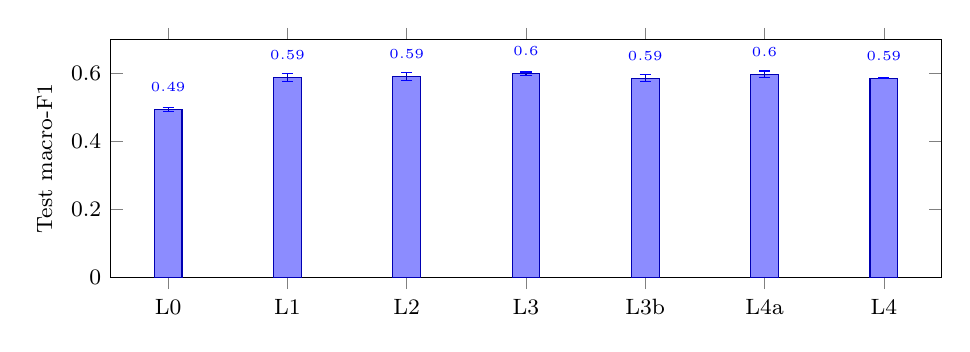
\begin{tikzpicture}
\begin{axis}[
  width=\columnwidth, height=4.6cm,
  ybar, bar width=10pt,
  ymin=0, ymax=0.7,
  ylabel={Test macro-F1},
  symbolic x coords={L0,L1,L2,L3,L3b,L4a,L4},
  xtick=data,
  nodes near coords, nodes near coords align={vertical},
  every node near coord/.append style={font=\tiny, yshift=3pt},
  tick label style={font=\footnotesize},
  label style={font=\footnotesize},
  enlarge x limits=0.08,
]
\addplot+[fill=blue!45, draw=blue!70!black,
  error bars/.cd, y dir=both, y explicit]
coordinates {
(L0,0.494) +- (0,0.006)
(L1,0.588) +- (0,0.012)
(L2,0.592) +- (0,0.012)
(L3,0.600) +- (0,0.005)
(L3b,0.587) +- (0,0.011)
(L4a,0.598) +- (0,0.010)
(L4,0.587) +- (0,0.001)
};
\end{axis}
\end{tikzpicture}
\caption{Task 2 ladder (mean $\pm$ s.d. over three seeds). Only L0$\rightarrow$L1 exceeds the noise.}
\label{fig:ladder}
\end{figure}

\textbf{Task~2.} Table~\ref{tab:ladder2} and Fig.~\ref{fig:ladder} list the rungs. The earlier version stripped a fixed prefix from image paths with \texttt{lstrip}, which removes a \emph{set of characters} rather than a prefix, so \texttt{iraq\_iran\_earthquake} became \texttt{raq\_iran\_earthquake}; this silently dropped both earthquake events, about 11\% of every split, from training and development data (L0). Restoring them (L1) raises test macro-F1 from \pmse{0.494}{0.006} to \pmse{0.588}{0.012}, a paired gain of \pmse{+0.095}{0.011} that is positive at every seed; the seed-42 bootstrap interval is $[+0.051, +0.149]$.

Every later step moves macro-F1 by less than the noise: $+0.004$ (QuickGELU, L2), $+0.008$ (10-epoch budget, L3), $-0.013$ (deterministic cached features, L3b), $+0.012$ (mixed precision, L4a) and $-0.011$ (randomly initialised text encoder, L4). The last rung reproduces the build as delivered at the start of this phase, whose DistilBERT was, through a construction bug, trained from random weights: the cosine similarity between its word embeddings and the pretrained ones is $-0.0002$. Its effect is no larger than the opposite-signed effect of mixed precision alone, so it is not established. The rest of the current design therefore delivers equal accuracy at about one seventh of the compute (9.8 instead of 66.4 minutes per run). The earlier version also selected the best of 30 development evaluations, each randomised by a random crop applied to development and test images, which inflated its development scores (L0--L2) by about 0.06 over test. Alongside these, mis-ordered Task~1 report labels and hash-order tie-breaking in the neighbour vote were corrected.

\textbf{Which data mattered.} Per-class analysis at seed 42 shows that 56\% of the summed per-class L0$\rightarrow$L1 gain comes from one class, \emph{injured or dead people}, whose F1 rises from 0.167 to 0.632; eight of its ten test rows come from the two earthquake events. \emph{Affected individuals} (+0.145) and \emph{rescue, volunteering or donation} (+0.105) also improve, as expected from restoring about 11\% of the training data. Section~\ref{sec:robust} reaches the same conclusion from an independent experiment.

\begin{table}[t]
\centering
\caption{Task 3 ladder (deterministic). All rungs are scored on the same 529 test queries.}
\label{tab:ladder3}
\footnotesize
\setlength{\tabcolsep}{3pt}
\begin{tabular}{llrcc}
\toprule
Rung & Index & Rows & Acc. & Macro-F1 \\
\midrule
L0 & earlier (incl.\ test, ``Don't know'') & 18,082 & 0.722 & 0.688 \\
L1 & test rows removed & 17,553 & 0.503 & 0.378 \\
L2 & ``Don't know'' rows removed & 2,997 & 0.677 & 0.504 \\
L3 & development rows removed & 2,468 & 0.675 & 0.509 \\
L4 & tweet siblings removed (5-NN) & 2,361 & 0.667 & 0.491 \\
Final & L4 index + logistic probe & 2,361 & 0.684 & 0.615 \\
\bottomrule
\end{tabular}
\end{table}

\textbf{Task~3.} Table~\ref{tab:ladder3} follows the nearest-neighbour index. The earlier index held all 18,082 annotated images, including the test images, and 80.5\% of its rows carried a ``Don't know'' label that never occurs in the official damage splits, mostly assigned to images that were never annotated for damage. With the test images in the index, all 529 test queries retrieved themselves among their five neighbours, giving 0.688 macro-F1. Removing them (L1) reveals the earlier version's real performance, 0.378. Removing the polluted labels recovers 0.504 (L2); dropping development images (L3) and same-tweet siblings (L4) gives 0.509 and 0.491, within the noise of 529 queries. The gain of the leakage-free 5-NN over the earlier version's real performance is +0.114 (bootstrap $[+0.064, +0.167]$), and the probe adds a further +0.123 (Section~\ref{sec:component}).

\subsection{Component Ablation}
\label{sec:component}

\begin{table}[t]
\centering
\caption{Task 2 component ablation (three seeds). Parameters are trainable; the frozen CLIP encoder is excluded.}
\label{tab:comp}
\footnotesize
\setlength{\tabcolsep}{3.5pt}
\begin{tabular}{lrcc}
\toprule
Variant & Params & Acc. & Macro-F1 \\
\midrule
Full model (L4a) & 67.4M & \pmse{0.799}{0.006} & \pmse{0.598}{0.010} \\
Text only & 66.6M & \pmse{0.486}{0.010} & \pmse{0.294}{0.014} \\
Image only & 0.2M & \pmse{0.788}{0.002} & \pmse{0.601}{0.005} \\
Concatenation, no attention & 66.8M & \pmse{0.796}{0.007} & \pmse{0.595}{0.009} \\
No text$\rightarrow$image block & 67.1M & \pmse{0.795}{0.005} & \pmse{0.570}{0.014} \\
\bottomrule
\end{tabular}
\end{table}

\textbf{Task~2 components.} Table~\ref{tab:comp} removes one component at a time. A 200k-parameter MLP on the cached CLIP vector matches the full model (image-only minus full: \pmse{+0.003}{0.009}; seed-42 bootstrap $[-0.036, +0.034]$), and concatenation without attention is also a tie ($-0.003$). The text stream alone reaches only 0.294, an established collapse. Removing the text-to-image block gives \pmse{-0.029}{0.024}, negative at every seed, which we regard as suggestive only: that block is a linear copy of the image, and the image-to-text block and the direct image path remain in the ablated model.

\textbf{Where does text help?} Since Task~2 predicts the image label, text can only help where it describes the same thing as the image. Table~\ref{tab:agree} splits the test set by whether the text and image labels agree (955 rows) or not (1,282 rows). On agreed rows the full model beats image-only by \pmse{+0.021}{0.004} accuracy, positive at every seed (seed-42 bootstrap $[+0.012, +0.038]$); on disagreed rows it gives $-0.014$ macro-F1, and the two effects largely cancel over the whole test set. Text-only accuracy on disagreed rows (0.338) is below always predicting the majority class (0.430), as expected when the tweet describes a different category from the label being scored.

\begin{table}[t]
\centering
\caption{Task 2 by text--image label agreement (three seeds). Macro-F1 averages the classes present in the subset.}
\label{tab:agree}
\footnotesize
\setlength{\tabcolsep}{3.5pt}
\begin{tabular}{llcc}
\toprule
Subset & Model & Acc. & Macro-F1 \\
\midrule
\multirow{4}{*}{Agreed (955)} & Full model & \pmse{0.866}{0.008} & \pmse{0.745}{0.026} \\
 & Image only & \pmse{0.845}{0.004} & \pmse{0.696}{0.031} \\
 & Text only & \pmse{0.685}{0.019} & \pmse{0.482}{0.061} \\
 & Majority class & 0.528 & 0.099 \\
\midrule
\multirow{4}{*}{Disagreed (1,282)} & Full model & \pmse{0.750}{0.005} & \pmse{0.549}{0.009} \\
 & Image only & \pmse{0.745}{0.005} & \pmse{0.563}{0.004} \\
 & Text only & \pmse{0.338}{0.005} & \pmse{0.198}{0.010} \\
 & Majority class & 0.430 & 0.075 \\
\bottomrule
\end{tabular}
\end{table}

\textbf{Task~3 classifier and embedding.} Table~\ref{tab:emb3} varies the embedding and the classifier on the same index and training rows. A logistic probe beats 5-NN voting on the fused embedding by +0.123 macro-F1 (bootstrap $[+0.062, +0.186]$) and on the image embedding by +0.087 ($[+0.028, +0.148]$), which motivated the hybrid design. The bootstrap resamples the 529 test queries for one index and one probe, so it does not cover training variability. Image-only retrieval (0.507) is not worse than the fused embedding (0.491), and text-only retrieval is clearly weaker (0.428). Varying $k \in \{1,3,5,10,20\}$ moves test macro-F1 between 0.454 and 0.515 with no established effect; $k=5$ is best on the development set (0.483). Similarity-weighted voting is identical to majority voting in all 15 combinations of embedding and $k$, because the neighbours' similarities are close together (mean gap between the first and fifth neighbour 0.046). Class-balanced voting raises development macro-F1 by 0.037 but test macro-F1 by only 0.004, while lowering accuracy from 0.667 to 0.586.

\begin{table}[t]
\centering
\caption{Task 3 embedding and classifier (deterministic; probe $C$ tuned on dev).}
\label{tab:emb3}
\footnotesize
\begin{tabular}{llccc}
\toprule
Embedding & Classifier & Dev F1 & Acc. & Macro-F1 \\
\midrule
Image & 5-NN & 0.543 & 0.675 & 0.507 \\
Image & logistic probe & 0.621 & 0.673 & 0.595 \\
Text & 5-NN & 0.402 & 0.607 & 0.428 \\
Text & logistic probe & 0.473 & 0.509 & 0.463 \\
Fused & 5-NN & 0.483 & 0.667 & 0.491 \\
Fused & logistic probe & 0.593 & 0.684 & 0.615 \\
\bottomrule
\end{tabular}
\end{table}

\subsection{Robustness}
\label{sec:robust}

\textbf{Missing modality.} Replacing the image with a grey image at test time collapses both Task~2 models to the majority-class score (0.080 and 0.081 macro-F1, within 0.002 of always predicting \emph{not humanitarian} at every seed), so the models cannot fall back on the text alone. Replacing the text with an empty string leaves the randomly initialised model unchanged (+0.003) but costs the current model 0.087 on average (range 0.058--0.103): the pretrained text stream is used, even though it adds no information the image lacks overall. Both inputs are out of distribution for their encoders, so part of each drop may reflect the input shift. For the Task~3 5-NN classifier, a grey image costs 0.039 and an empty text 0.052.

\textbf{Leave-one-disaster-out.} We trained (or built the index) on six events and tested on the seventh, asserting that the held-out event contributes no training or development rows. Task~2 uses the image-only model, which ties the full model overall, as a proxy, with three seeds per fold and checkpoints selected on the other events' development rows. Table~\ref{tab:lodo} compares each fold with the standard model on the same rows.

\begin{table*}[t]
\centering
\caption{Leave-one-disaster-out macro-F1 (held out / in-distribution). Per-event macro-F1 averages the classes present in that event, so the averages differ from the pooled scores. Task 2 uses the image-only model (three seeds); Task 3 and the Task 1 TF-IDF column are deterministic; $^{\dagger}$ Task 1 BERTweet is a single seed (42) per fold, selected on the other events' development rows.}
\label{tab:lodo}
\footnotesize
\begin{tabular}{lrrcccc}
\toprule
Held-out event & T2 test rows & T3 test rows & T1 TF-IDF & T1 BERTweet$^{\dagger}$ & T2 (image, $n$=3) & T3 (5-NN) \\
\midrule
California wildfires & 216 & 87 & 0.615 / 0.606 & 0.662 / 0.637 & 0.664 / 0.691 & 0.309 / 0.315 \\
Hurricane Harvey & 572 & 132 & 0.735 / 0.758 & 0.809 / 0.824 & 0.590 / 0.599 & 0.481 / 0.494 \\
Hurricane Irma & 559 & 120 & 0.675 / 0.697 & 0.743 / 0.738 & 0.534 / 0.536 & 0.271 / 0.483 \\
Hurricane Maria & 518 & 133 & 0.692 / 0.742 & 0.793 / 0.808 & 0.526 / 0.542 & 0.389 / 0.343 \\
Iraq--Iran earthquake & 73 & 23 & 0.622 / 0.625 & 0.665 / 0.716 & 0.421 / 0.558 & 0.293 / 0.302 \\
Mexico earthquake & 176 & 21 & 0.628 / 0.638 & 0.665 / 0.749 & 0.568 / 0.660 & 0.462 / 0.417 \\
Sri Lanka floods & 123 & 13 & 0.793 / 0.932 & 0.978 / 0.955 & 0.700 / 0.711 & 0.273 / 0.316 \\
\midrule
Average over events & 2,237 & 529 & 0.680 / 0.714 & 0.759 / 0.775 & 0.572 / 0.614 & 0.354 / 0.381 \\
\bottomrule
\end{tabular}
\end{table*}

Task~1 with TF-IDF loses 0.034 on average, concentrated in the Sri Lanka floods (0.932 to 0.793), the only flood event; the BERTweet model (one seed per fold) loses 0.016 on average, most on the Mexico earthquake (0.749 to 0.665); with one seed per fold the per-event numbers are indicative only. Task~2 loses most on the two earthquakes (Iraq--Iran $-0.137$, Mexico $-0.092$), while the hurricanes and the flood change by less than 0.02; the wildfire change ($-0.026$) is within its seed spread ($\pm0.099$). Pooled over all rows, the Task~2 drop at seed 42 is $-0.073$ (bootstrap $[-0.108, -0.036]$), larger than the per-event average because macro-F1 weights classes equally: 0.052 of it comes from \emph{injured or dead people}, whose F1 falls from 0.609 to 0.190, and without that 10-row class the drop is $-0.020$. This matches the ladder: without earthquake data that class scores 0.167 (L0) and 0.190 (here); with it, 0.632 (L1) and 0.609 (in-distribution). Task~3 changes are mixed in sign, and three events have only 13--23 test images, so they are indicative only. Text and image fail on different unseen events: text on the flood, images on the earthquakes. \todo{With BERTweet (single seed) the flood is no longer the text model's weak event (held out 0.978 against 0.955 in distribution, 107 rows); its largest losses are on the earthquakes. Rewrite this sentence.}

\subsection{Confidence and Calibration}
\label{sec:calib}

\begin{table}[t]
\centering
\caption{Calibration on the test set before and after temperature scaling ($T$ fitted on dev). The tool uses the seed-42 Task 2 checkpoint and its temperature.}
\label{tab:calib}
\footnotesize
\setlength{\tabcolsep}{3.5pt}
\begin{tabular}{lccccc}
\toprule
Model & Acc. & Mean conf. & ECE & $T$ & ECE after \\
\midrule
T2, seed 42 & 0.803 & 0.843 & 0.046 & 1.185 & 0.024 \\
T2, seed 43 & 0.803 & 0.879 & 0.077 & 1.467 & 0.022 \\
T2, seed 44 & 0.792 & 0.878 & 0.087 & 1.472 & 0.025 \\
T3 probe & 0.684 & 0.607 & 0.077 & 0.693 & 0.038 \\
\midrule
T1, seed 42 & 0.835 & 0.879 & 0.045 & 1.283 & 0.026 \\
T1, seed 43 & 0.846 & 0.881 & 0.039 & 1.194 & 0.032 \\
T1, seed 44 & 0.840 & 0.888 & 0.049 & 1.343 & 0.022 \\
T1, deployed & 0.848 & 0.936 & 0.088 & 1.825 & 0.044 \\
\bottomrule
\end{tabular}
\end{table}

Table~\ref{tab:calib} reports the expected calibration error. The Task~2 model is over-confident and the Task~3 probe under-confident; temperature scaling brings both below 0.04. The Task~1 BERTweet model is over-confident too (deployed checkpoint: test mean confidence 0.936 against accuracy 0.848, ECE 0.088); scaling with $T=1.825$ lowers its ECE to 0.044 (the three seeds reach 0.022--0.032), which is above the 0.04 reached for Tasks~2 and~3. Both confidence signals in Task~3 track correctness. By probe-confidence quintile, test accuracy rises from 0.500 to 0.575, 0.623, 0.811 and 0.914. When the probe and the five neighbours agree (345 queries) accuracy is 0.812; when they disagree (184) it is 0.446 for the probe and 0.397 for the neighbours, so disagreement marks hard cases rather than identifying the better method. The area under the ROC curve for predicting a correct answer is 0.718 for confidence ($[0.672, 0.762]$) and 0.692 for agreement ($[0.650, 0.735]$). The two signals are partly independent: among agreeing queries, accuracy ranges from 0.672 at low confidence to 0.894 at high confidence.

\subsection{Image Encoder Scale}
\label{sec:scale}
Because the image carries most of the signal, we replaced CLIP ViT-B/32 with ViT-L/14, keeping everything else fixed (Table~\ref{tab:scale}). The two encoders differ in both size (an image tower of 304M against 88M parameters) and patch size (14 against 32 pixels), so any gain is attributed to the larger CLIP model, not to size alone. For Task~2, the image-only model improves from 0.601 to 0.644 on average, positive at every seed (seed-42 bootstrap $[+0.001, +0.063]$, which only just excludes zero); feeding the raw L/14 features gives 0.648 and $[+0.017, +0.081]$, so normalisation does not explain the gain. Against the full B/32 fusion model the difference is not established. For Task~3 the larger encoder helps the image-only paths but neither fused comparison is established. Zero-shot macro-F1 rises from 0.299 to 0.372, but under development-calibrated biases the ranking of the two encoders reverses (0.397 for B/32 against 0.365 for L/14), so only the statement that both are far below a trained probe is robust.

\begin{table}[t]
\centering
\caption{CLIP ViT-B/32 against ViT-L/14 (test macro-F1). $\Delta$: paired bootstrap at seed 42 (T2) or over the 529 queries (T3), L/14 minus B/32.}
\label{tab:scale}
\footnotesize
\setlength{\tabcolsep}{3pt}
\begin{tabular}{lccc}
\toprule
Setting & B/32 & L/14 & $\Delta$ [95\% CI] \\
\midrule
T2 image only ($n$=3) & 0.601 & 0.644 & +0.031 [+0.001, +0.063] \\
T2 L/14 image only vs.\ L4a & 0.598 & 0.644 & +0.029 [$-$0.010, +0.071] \\
T3 fused, logistic probe & 0.615 & 0.607 & $-$0.008 [$-$0.044, +0.030] \\
T3 fused, 5-NN & 0.491 & 0.505 & +0.014 [$-$0.035, +0.063] \\
T3 image, logistic probe & 0.595 & 0.621 & -- \\
T3 image, 5-NN & 0.507 & 0.548 & -- \\
T3 zero-shot & 0.299 & 0.372 & -- \\
T3 zero-shot, calibrated bias & 0.397 & 0.365 & -- \\
\bottomrule
\end{tabular}
\end{table}

\subsection{Class Imbalance}
\label{sec:imbalance}
The class weighting used throughout had never been compared with not using it. Table~\ref{tab:imb} compares ten treatments on the image-only head over cached CLIP features, for both encoders. On development data seven of the ten arms are tied with the best on both encoders; the rule fixed in advance (highest development balanced accuracy among the tied arms) picks inverse-frequency weighting on B/32 and focal loss with inverse-frequency weights on L/14. Because the encoders disagree, no new loss is adopted. The rule has little power, since development holds only 8 \emph{injured or dead} and 2 \emph{missing or found} rows, so this does not show that inverse-frequency weighting is the best choice.

\begin{table}[t]
\centering
\caption{Task 2 class-imbalance treatments, image-only head, three seeds. Test F1 is the seed mean; Bal.\ is test balanced accuracy.}
\label{tab:imb}
\footnotesize
\setlength{\tabcolsep}{3pt}
\begin{tabular}{lcccccc}
\toprule
 & \multicolumn{3}{c}{CLIP B/32} & \multicolumn{3}{c}{CLIP L/14} \\
\cmidrule(lr){2-4}\cmidrule(lr){5-7}
Arm & Dev F1 & Test F1 & Bal. & Dev F1 & Test F1 & Bal. \\
\midrule
None & 0.596 & 0.608 & 0.579 & 0.624 & 0.653 & 0.636 \\
Inverse freq.\ (used) & 0.568 & 0.601 & 0.651 & 0.612 & 0.644 & 0.693 \\
Sqrt inverse freq. & 0.589 & 0.614 & 0.626 & 0.629 & 0.654 & 0.677 \\
Effective number~\cite{cui2019} & 0.587 & 0.617 & 0.629 & 0.629 & 0.656 & 0.676 \\
Focal, $\gamma$=1 & 0.599 & 0.608 & 0.582 & 0.632 & 0.652 & 0.637 \\
Focal, $\gamma$=2 & 0.602 & 0.612 & 0.590 & 0.630 & 0.652 & 0.638 \\
Focal $\gamma$=2 + inv. & 0.547 & 0.579 & 0.653 & 0.606 & 0.608 & 0.702 \\
Weighted sampler & 0.554 & 0.577 & 0.650 & 0.589 & 0.620 & 0.696 \\
Logit adjustment~\cite{menon2021} & 0.523 & 0.562 & 0.667 & 0.572 & 0.593 & 0.691 \\
None + post-hoc adj. & 0.596 & 0.610 & 0.587 & 0.627 & 0.651 & 0.652 \\
\bottomrule
\end{tabular}
\end{table}

Against no weighting, inverse-frequency weighting raises test balanced accuracy by +0.072 (B/32) and +0.057 (L/14) and \emph{vehicle damage} recall by +0.222 and +0.111, with paired intervals excluding zero, while the macro-F1 difference is not distinguishable ($-0.007$ and $-0.010$). Weighted sampling, focal loss with inverse-frequency weights and logit adjustment are each worse than inverse-frequency weighting in macro-F1 on both encoders. The effective-number weights have the highest test macro-F1 but were not selected on development data, and their advantage over inverse-frequency weighting is borderline (lower interval bounds +0.0003 and +0.0010), so we do not read it as an improvement. \emph{Missing or found people} has F1 = 0 under every treatment, so no loss-level treatment lifts the 0.875 cap.

A separate check, fixed in advance, asked whether weighting matters inside a fusion model, using the L4a recipe with L/14 features. Removing weighting lowers balanced accuracy on development ($-0.050$, $[-0.070, -0.030]$) and test ($-0.057$), and lowers \emph{injured or dead} recall on both, while macro-F1 does not change beyond noise (test $-0.014$, $[-0.040, +0.009]$). Inverse-frequency weighting is therefore retained. \textbf{Task~1 (post-hoc).} The same question for the Task~1 BERTweet model (three seeds, development decides) shows that weighting raises the dev balanced accuracy by +0.0175 (paired 95\% interval [+0.0095, +0.0258]) by raising the recall of \emph{not informative} (0.670 against 0.604 on development data) at the cost of the recall of \emph{informative} (0.895 against 0.926) and of the precision on the minority class (Table~\ref{tab:weight1}). Weighted F1 and macro-F1 were not tested with a bootstrap; their means differ by less than the seed spread. This is a different operating point, not a safety improvement; whether it is preferable depends on the cost of a missed informative tweet.

\begin{table}[t]
\centering
\caption{Task 1 loss weighting for BERTweet (post-hoc arm; mean of three seeds). Weighting trades precision for recall on the minority class; it is a different operating point, not a safety improvement.}
\label{tab:weight1}
\footnotesize
\setlength{\tabcolsep}{3pt}
\begin{tabular}{lcccc}
\toprule
 & \multicolumn{2}{c}{Dev} & \multicolumn{2}{c}{Test} \\
\cmidrule(lr){2-3}\cmidrule(lr){4-5}
Metric & weighted & unweighted & weighted & unweighted \\
\midrule
Not-informative recall & 0.670 & 0.604 & 0.681 & 0.625 \\
Informative recall & 0.895 & 0.926 & 0.902 & 0.933 \\
Not-informative precision & 0.714 & 0.763 & 0.732 & 0.785 \\
\bottomrule
\end{tabular}
\end{table}


\subsection{Architecture and Fine-Tuning Choices}
\label{sec:arch}
We compared image backbones, text encoders, fusion heads and hyperparameters on frozen cached features, and fine-tuned fusion against a frozen head, each with the selection rule of Section~\ref{sec:protocol} (Table~\ref{tab:arch}). Tied means that no difference is resolvable on development data, not that the arms are equal, so the many ties reflect limited power.

\begin{table*}[t]
\centering
\caption{Task 2 design choices on frozen features (three seeds): the pick of the pre-set rule, the best arm on development (mean dev macro-F1), the best arm minus the pick with its paired development 95\% interval, and the basis of the pick.}
\label{tab:arch}
\footnotesize
\setlength{\tabcolsep}{4pt}
\begin{tabular}{lllll}
\toprule
Decision & Pick & Best arm on dev & Best minus pick [95\% CI] & Basis \\
\midrule
Image backbone & CLIP L/14 & CLIP L/14 (0.612) & best arm & resolvable \\
Text encoder & MiniLM & MPNet (0.294) & +0.010 [$-$0.002, +0.022] & tie-break \\
Head & image only & image only (0.612) & best arm & tie-break (heads tied) \\
Loss & inverse frequency & focal loss (0.632) & +0.020 [$-$0.012, +0.048] & default kept \\
Hyperparameters & lr $10^{-4}$, dropout 0.2, $d$ 128 & lr $3{\times}10^{-4}$, dropout 0.1, $d$ 512 (0.620) & +0.012 [$-$0.011, +0.035] & tie-break \\
Fine-tuned vs.\ frozen & frozen head & MiniLM fine-tuned (0.610) & +0.002 [$-$0.016, +0.020] & tie-break \\
\bottomrule
\end{tabular}
\end{table*}

\textbf{Image backbone.} CLIP L/14 is the only choice resolvable on development data: every alternative is worse, and the test means follow the same order (CLIP L/14 0.644, CLIP B/32 0.601, DINOv2 0.585, ResNet-50 0.527).

\textbf{Text and head.} Frozen sentence encoders alone score about 0.29 to 0.30 test macro-F1 (MiniLM 0.285, MPNet 0.299), in line with the fine-tuned DistilBERT text-only model (0.294). Concatenation, gated late fusion, cross-attention and the image-only head are tied on development data (test 0.654, 0.640, 0.639 and 0.644). This cross-attention result holds for frozen MiniLM token features and does not test fine-tuned text.

\textbf{Hyperparameters.} 26 of 27 grid configurations are tied. The configuration with the best development score (model width 512) scores below the default on test (0.634 against 0.644), consistent with selecting on development noise.

\textbf{Fine-tuned fusion.} Fine-tuned DistilBERT (67.4M trainable parameters) and fine-tuned MiniLM (23.7M) fused with L/14 features are tied with the frozen image-only head (116k) on development data, and their test macro-F1 (0.635 and 0.648 against 0.635) is not distinguishable. The arms differ in head and recipe as well as text, and the DistilBERT arm reuses earlier runs, so this is not a blind comparison.

\textbf{Outcome.} The rules select frozen CLIP L/14 features with an image-only head and inverse-frequency loss, with test macro-F1 0.635 (test-sampling interval 0.598 to 0.663). This is the simplest model within noise of the best, not a win over the fusion model: the intervals overlap and the setups differ. We therefore keep L4a as the deployed model, since it is within noise of this pick and its text stream gives an established gain on the rows where text and image agree, and we record the larger image encoder as the most promising upgrade.

\subsection{What Is Established}
With three seeds, a seed noise floor of about 0.01 and paired bootstrap intervals, we regard the following as established: the gain from restoring the earthquake data in Task~2; the dependence of \emph{injured or dead people} on that data, seen in two independent experiments; the fall of the earlier Task~3 score once self-retrieval is removed, and the gain of the leakage-free system over it; the gain of the probe over 5-NN voting; the collapse of the text-only model; the accuracy gain of the full Task~2 model over image-only on rows where the labels agree; the collapse of every Task~2 model without its image; the gain of the ViT-L/14 image-only model; and the gains in balanced accuracy and rare-class recall from inverse-frequency weighting. Differences of about 0.01 between Task~2 configurations, including the effects of mixed precision and random initialisation, the whole-set comparison of image-only, concatenation and the full model, and the differences among Task~3 rungs L2 to L4, are not established.

\textbf{Day~4, established.} BERTweet over TF-IDF with logistic regression for Task~1 on development data (+0.0195 weighted F1, interval [+0.0049, +0.0340], positive at every seed; the lower bound is small); the effect of Task~1 loss weighting on the recall of the minority class; and, as a secondary result, the worse development weighted F1 of the guide's core model than L4a ($-$0.0341, interval [$-$0.0484, $-$0.0200]).

\textbf{Day~4, not established.} the BiLSTM against TF-IDF with logistic regression (+0.0005 [$-$0.0129, +0.0133]); fusion against text-only for Task~1 (best development gain +0.0043); the core model against L4a and against the image-only CLIP B/32 head on development macro-F1; BERTweet against DistilBERT as the Task~2 text encoder (+0.0165, interval [$-$0.0004, +0.0334]); BERTweet with CLIP B/32 against L4a; the effect of the duplicates; and the agreed/disagreed differences, which are descriptive (no interval). All of these are exploratory (about twenty further comparisons, no multiplicity correction); development data decide and test is reported afterwards.

% =====================================================================

\subsection{Model Exploration for Tasks~1 and~2}
\label{sec:explore}
At our guide's request we compared the candidate models of the two task lists (Task~1: TF-IDF with logistic regression, naive Bayes or a random forest, a BiLSTM with GloVe, BERTweet, image heads on ResNet50, DINOv2 and CLIP, late and early fusion; Task~2: the same families plus DistilBERT and the Task~2 fusion designs). The candidate lists, the selection rules and the comparisons below were committed before the runs
(\texttt{SELECTION\_RULE\_DAY4.md}); arms added after seeing earlier results are marked $^\ast$. Development data decide, the test split is scored once, ties go to the model with the fewest trainable parameters, every neural model has three seeds, and no multiplicity correction is applied to the roughly twenty added comparisons.
Provenance fields stored with every run (task, label column, hash of the training split, initialisation) guard against using weights trained on another task (Section~\ref{sec:data_integrity}).

\textbf{Task~1.} Table~\ref{tab:t1explore} and Fig.~\ref{fig:t1models} list the models. All image heads score against the text label, so they are far below the text models (0.761 for the best head against 0.838 for BERTweet; the majority class scores 0.604). The class-weighted classical text models (logistic regression, balanced naive Bayes, Complement NB, random forest, linear SVM) plateau between 0.786 and 0.811 development weighted F1; naive Bayes needs class weights
(macro-F1 0.588 unweighted against 0.737 balanced). The BiLSTM is tied with TF-IDF and logistic regression (+0.0005 [$-$0.0129, +0.0133] on development weighted F1; post-hoc). BERTweet is best on development data, and the rule fixed in advance (switch if the paired development interval of the seed-averaged gain excludes zero and the gain is positive at every seed) is met
(+0.0195 [+0.0049, +0.0340]; per seed +0.0212, +0.0182, +0.0191), so BERTweet replaced TF-IDF as the deployed Task~1 model; the lower bound is small, the test gap is larger (0.838 against 0.797). Latency is not a reason to keep TF-IDF (Table~\ref{tab:latency}).
Table~\ref{tab:weight1} shows what loss weighting does (Section~\ref{sec:imbalance}).

\begin{table*}[t]
\centering
\caption{Task 1 (informative or not) scored against the text label, sorted by development weighted F1. Mean\,$\pm$\,s.d.\ over three seeds where $n$=3; the TF-IDF models and the majority class are single deterministic runs. $^\ast$ post-hoc arm, added after the first Day~4 results (Section~\ref{sec:protocol}). The majority class always predicts \emph{informative}.}
\label{tab:t1explore}
\footnotesize
\setlength{\tabcolsep}{3pt}
\begin{tabular}{lcccccccc}
\toprule
Model & $n$ & Dev W-F1 & Test acc. & Test W-F1 & Test macro-F1 & Bal.\ acc. & MCC & ROC-AUC \\
\midrule
BERTweet + CLIP L/14 (concat) & 3 & \pmse{0.835}{0.002} & \pmse{0.847}{0.008} & \pmse{0.845}{0.006} & \pmse{0.805}{0.005} & \pmse{0.797}{0.007} & \pmse{0.612}{0.014} & \pmse{0.898}{0.003} \\
Late fusion, BERTweet + CLIP L/14 & 3 & \pmse{0.835}{0.002} & \pmse{0.845}{0.004} & \pmse{0.845}{0.002} & \pmse{0.806}{0.002} & \pmse{0.804}{0.006} & \pmse{0.613}{0.003} & \pmse{0.884}{0.003} \\
Core model: BERTweet + ResNet50 & 3 & \pmse{0.834}{0.002} & \pmse{0.846}{0.003} & \pmse{0.844}{0.003} & \pmse{0.805}{0.003} & \pmse{0.800}{0.004} & \pmse{0.611}{0.006} & \pmse{0.896}{0.001} \\
BERTweet, weighted CE & 3 & \pmse{0.830}{0.002} & \pmse{0.840}{0.005} & \pmse{0.838}{0.002} & \pmse{0.797}{0.001} & \pmse{0.791}{0.011} & \pmse{0.597}{0.003} & \pmse{0.897}{0.001} \\
BERTweet, unweighted CE$^\ast$ & 3 & \pmse{0.830}{0.004} & \pmse{0.847}{0.003} & \pmse{0.841}{0.005} & \pmse{0.797}{0.008} & \pmse{0.779}{0.012} & \pmse{0.603}{0.011} & \pmse{0.895}{0.002} \\
BiLSTM + GloVe & 3 & \pmse{0.811}{0.003} & \pmse{0.810}{0.013} & \pmse{0.811}{0.010} & \pmse{0.766}{0.008} & \pmse{0.768}{0.003} & \pmse{0.534}{0.016} & \pmse{0.858}{0.007} \\
TF-IDF + LR (v2) & 1 & 0.811 & 0.794 & 0.797 & 0.751 & 0.758 & 0.504 & 0.841 \\
NB, balanced weights$^\ast$ & 1 & 0.799 & 0.787 & 0.788 & 0.737 & 0.737 & 0.473 & 0.839 \\
Random Forest & 1 & 0.798 & 0.818 & 0.808 & 0.751 & 0.732 & 0.517 & 0.835 \\
Linear SVM & 1 & 0.794 & 0.802 & 0.791 & 0.729 & 0.711 & 0.473 & 0.825 \\
Complement NB$^\ast$ & 1 & 0.786 & 0.808 & 0.789 & 0.720 & 0.696 & 0.480 & 0.840 \\
CLIP L/14 head (image) & 3 & \pmse{0.763}{0.006} & \pmse{0.755}{0.007} & \pmse{0.761}{0.006} & \pmse{0.712}{0.005} & \pmse{0.726}{0.004} & \pmse{0.430}{0.009} & \pmse{0.797}{0.000} \\
DINOv2 head (image) & 3 & \pmse{0.719}{0.005} & \pmse{0.707}{0.007} & \pmse{0.718}{0.006} & \pmse{0.668}{0.006} & \pmse{0.690}{0.004} & \pmse{0.352}{0.009} & \pmse{0.743}{0.002} \\
ResNet50 head (image) & 3 & \pmse{0.711}{0.005} & \pmse{0.692}{0.013} & \pmse{0.702}{0.009} & \pmse{0.644}{0.006} & \pmse{0.658}{0.004} & \pmse{0.297}{0.007} & \pmse{0.721}{0.003} \\
NB, unweighted (reference) & 1 & 0.698 & 0.767 & 0.708 & 0.588 & 0.591 & 0.342 & 0.840 \\
Majority class & 1 & 0.604 & 0.721 & 0.604 & 0.419 & 0.500 & 0.000 & 0.500 \\
\bottomrule
\end{tabular}
\end{table*}

\begin{figure}[t]
\centering
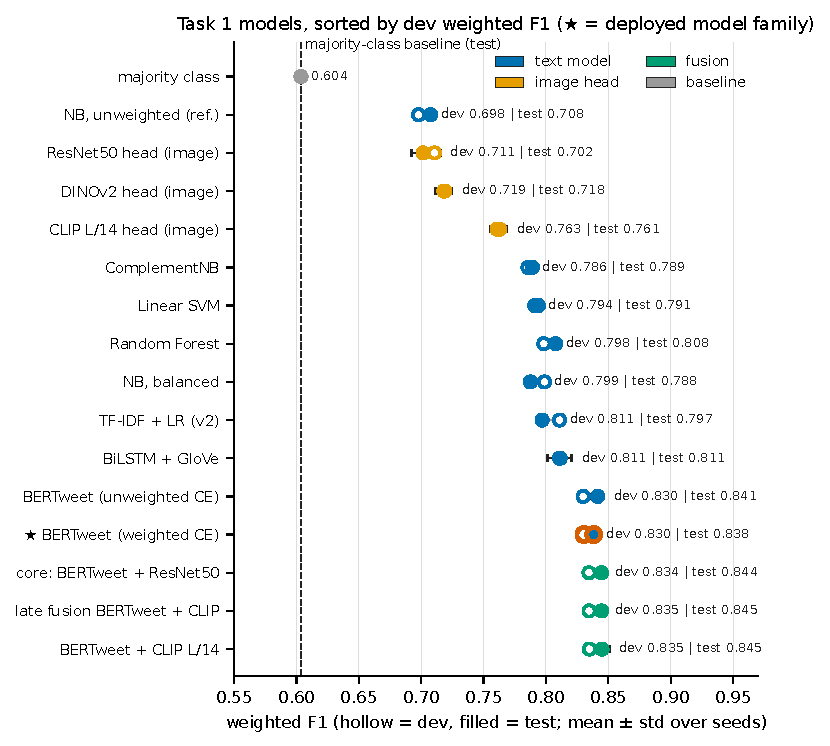
\includegraphics[width=\columnwidth]{figures/fig_c4_t1_models.pdf}
\caption{Task~1 models by development weighted F1 (hollow: development, filled: test; whiskers: s.d.\ over seeds; dashed: majority class on the test split; $\bigstar$: the deployed model family).}
\label{fig:t1models}
\end{figure}

\textbf{Fusion for Task~1.} Late fusion of BERTweet with the CLIP L/14 head, the guide's core model (BERTweet with frozen ResNet50 features) and a BERTweet and CLIP L/14 concatenation all gain 0.0040 to 0.0043 weighted F1 on development data over the better single model, positive at every seed but not distinguishable from BERTweet alone (best fused minus text-only
+0.0043 [$-$0.0018, +0.0102]); the three fused models tie with each other on development data (a spread of 0.0003), so none is best, and the tie goes to the text-only model. On the test split the intervals exclude zero narrowly (Table~\ref{tab:prereg}); test does not decide.
Late fusion has a lower test ROC-AUC than BERTweet alone (0.884 against 0.897); equal-weight averaging with a weaker image model plausibly degrades the ranking (not tested).
\todo{Decide whether the ROC-AUC explanation stays or is cut.}

\textbf{Task~2.} Table~\ref{tab:t2explore} and Fig.~\ref{fig:t2models} list the Task~2 models. The classical text models reach 0.278 test macro-F1 at best and DistilBERT 0.294; BERTweet reaches 0.308 with the DistilBERT recipe (dev 0.311 against 0.295), consistent at every seed on development data,
but the paired development interval marginally includes zero [$-$0.0004, +0.0334]: small, not robust; the input differs (BERTweet reads the raw tweet, DistilBERT the cleaned text), which is a confound. Every text-only model is far below the image heads (0.601 for CLIP B/32 and 0.644 for L/14).

\begin{table*}[t]
\centering
\caption{Task 2 (eight humanitarian classes) scored against the image label. Mean\,$\pm$\,s.d.\ over three seeds (the TF-IDF models and the majority class are single runs). $^\ast$ post-hoc. The majority-class top-2 value is arbitrary (a constant predictor ties every other class) and is not meaningful.}
\label{tab:t2explore}
\footnotesize
\setlength{\tabcolsep}{3pt}
\begin{tabular}{lccccccc}
\toprule
Model & Dev macro-F1 & Test macro-F1 & Test W-F1 & Test acc. & Bal.\ acc. & MCC & Top-2 \\
\midrule
Majority class (\emph{not humanitarian}) & 0.082 & 0.080 & 0.302 & 0.472 & 0.125 & 0.000 & -- \\
TF-IDF + LR, class-weighted & 0.270 & 0.278 & 0.475 & 0.457 & 0.357 & 0.288 & 0.687 \\
TF-IDF + LinearSVC, class-weighted & 0.227 & 0.227 & 0.503 & 0.549 & 0.223 & 0.293 & 0.755 \\
Complement NB, unweighted (reference) & 0.238 & 0.248 & 0.522 & 0.546 & 0.246 & 0.315 & 0.736 \\
Complement NB, balanced weights$^\ast$ & 0.216 & 0.213 & 0.364 & 0.318 & 0.323 & 0.196 & 0.553 \\
DistilBERT, text only & \pmse{0.295}{0.005} & \pmse{0.294}{0.014} & \pmse{0.499}{0.008} & \pmse{0.486}{0.010} & \pmse{0.320}{0.020} & \pmse{0.308}{0.010} & \pmse{0.726}{0.005} \\
BERTweet, text only (DistilBERT-matched recipe) & \pmse{0.311}{0.001} & \pmse{0.308}{0.018} & \pmse{0.526}{0.012} & \pmse{0.508}{0.013} & \pmse{0.360}{0.007} & \pmse{0.344}{0.014} & \pmse{0.731}{0.022} \\
BERTweet, text only (4-epoch recipe) & \pmse{0.308}{0.003} & \pmse{0.301}{0.005} & \pmse{0.507}{0.005} & \pmse{0.476}{0.004} & \pmse{0.390}{0.005} & \pmse{0.325}{0.005} & \pmse{0.684}{0.005} \\
Image head, CLIP B/32 & \pmse{0.568}{0.008} & \pmse{0.601}{0.005} & \pmse{0.793}{0.002} & \pmse{0.788}{0.002} & \pmse{0.651}{0.002} & \pmse{0.708}{0.002} & \pmse{0.944}{0.001} \\
Image head, CLIP L/14 & \pmse{0.612}{0.002} & \pmse{0.644}{0.009} & \pmse{0.816}{0.004} & \pmse{0.812}{0.004} & \pmse{0.693}{0.007} & \pmse{0.740}{0.005} & \pmse{0.944}{0.002} \\
L4a: CLIP B/32 + DistilBERT cross-attention (deployed) & \pmse{0.585}{0.008} & \pmse{0.598}{0.010} & \pmse{0.800}{0.006} & \pmse{0.799}{0.006} & \pmse{0.610}{0.008} & \pmse{0.717}{0.009} & \pmse{0.940}{0.003} \\
Late fusion, BERTweet + CLIP L/14 head & \pmse{0.597}{0.003} & \pmse{0.622}{0.007} & \pmse{0.804}{0.003} & \pmse{0.800}{0.003} & \pmse{0.691}{0.008} & \pmse{0.723}{0.005} & \pmse{0.920}{0.002} \\
Core model: BERTweet + ResNet50 (frozen) & \pmse{0.561}{0.010} & \pmse{0.553}{0.004} & \pmse{0.751}{0.015} & \pmse{0.748}{0.019} & \pmse{0.587}{0.018} & \pmse{0.653}{0.013} & \pmse{0.914}{0.008} \\
BERTweet + CLIP B/32 (frozen)$^\ast$ & \pmse{0.571}{0.002} & \pmse{0.606}{0.010} & \pmse{0.798}{0.006} & \pmse{0.793}{0.006} & \pmse{0.646}{0.012} & \pmse{0.714}{0.008} & \pmse{0.940}{0.001} \\
\bottomrule
\end{tabular}
\end{table*}

\begin{figure}[t]
\centering
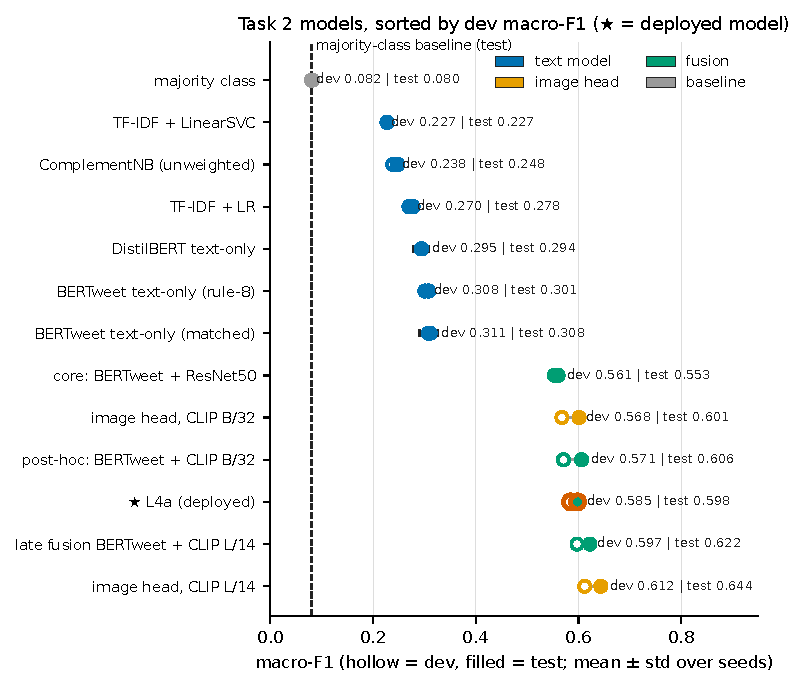
\includegraphics[width=\columnwidth]{figures/fig_c5_t2_models.pdf}
\caption{Task~2 models by development macro-F1 (hollow: development, filled: test; whiskers: s.d.\ over seeds; dashed: majority class; $\bigstar$: the deployed model).}
\label{fig:t2models}
\end{figure}

\textbf{The guide's core model.} BERTweet with frozen ResNet50 features reaches 0.553 test macro-F1, below L4a (0.598) and the image-only CLIP B/32 head (0.601). On the headline development macro-F1 neither difference is distinguishable
($-$0.0243 [$-$0.0579, +0.0064] against L4a; $-$0.0074 [$-$0.0428, +0.0246] against the image-only head), so the tie-break picks the model with fewer trainable parameters
(67,352,840 for L4a, 199,688 for the head, 135,755,784 for the core model); development weighted F1, a secondary metric, is worse for the core model in both comparisons and is corroboration only. The guide's architecture is therefore not adopted.
A post-hoc arm changes only the frozen image backbone: BERTweet with frozen CLIP B/32 features (same text encoder, fusion head structure and recipe; the input projection of the image features changes width) reaches 0.606 test macro-F1. Swapping only the image backbone raises the guide's architecture to a level not distinguishable from L4a's
($-$0.0139 [$-$0.0317, +0.0025] on development macro-F1); the deficit is consistent with ResNet50, resolved on development weighted F1 (+0.0294 [+0.0155, +0.0437]) but not on development macro-F1
(+0.0104 [$-$0.0192, +0.0434]). The arm swaps the backbone against the core model but also changes text encoder and fusion head against L4a, so it is not an encoder-only test.

\begin{table*}[t]
\centering
\caption{Comparisons of the model exploration. The development difference decides; the test difference is reported afterwards and decides nothing. Paired bootstrap, seed-averaged, 10,000 resamples; ``not distinguishable'' means the 95\% interval includes zero. Dev weighted F1 for the two core-model comparisons is worse for the core model (Section~\ref{sec:explore}) and is corroboration only.}
\label{tab:prereg}
\footnotesize
\setlength{\tabcolsep}{4pt}
\begin{tabular}{p{5.6cm}p{3.3cm}p{2.3cm}p{3.2cm}p{3.0cm}}
\toprule
Comparison & Dev difference [95\% CI] & Dev verdict & Test difference (reporting only) & Basis \\
\midrule
Switch rule: BERTweet $-$ TF-IDF + LR (T1, W-F1) & +0.020 [+0.005, +0.034] & better (every seed) & +0.041 (point) & dev rule: switch \\
Best fused $-$ BERTweet text-only (T1, W-F1) & +0.004 [$-$0.002, +0.010] & not distinguishable & +0.007 [+0.001, +0.012] & tie $\rightarrow$ simpler: text-only \\
Core model $-$ L4a (T2, macro-F1) & $-$0.024 [$-$0.058, +0.006] & not distinguishable & $-$0.045 [$-$0.073, $-$0.016] & tie $\rightarrow$ fewer parameters: L4a \\
Core model $-$ image-only CLIP B/32 head (T2, macro-F1) & $-$0.007 [$-$0.043, +0.025] & not distinguishable & $-$0.048 [$-$0.080, $-$0.015] & tie $\rightarrow$ fewer parameters: image-only head \\
Post-hoc: BERTweet + CLIP B/32 $-$ core model (backbone swap only) (T2, macro-F1) & +0.010 [$-$0.019, +0.043] & not distinguishable & +0.053 [+0.027, +0.079] & post-hoc, descriptive \\
Post-hoc: BERTweet + CLIP B/32 $-$ L4a (T2, macro-F1) & $-$0.014 [$-$0.032, +0.003] & not distinguishable & +0.008 [$-$0.018, +0.034] & post-hoc, descriptive \\
Post-hoc: BERTweet text $-$ DistilBERT text (T2, macro-F1) & +0.017 [$-$0.000, +0.033] & not distinguishable & +0.014 [$-$0.007, +0.035] & post-hoc, descriptive \\
\bottomrule
\end{tabular}
\end{table*}

\textbf{Fusion gain.} Table~\ref{tab:fgain} and Fig.~\ref{fig:fgain} give the fusion gain over the better of the models a fused model is built from, and over the best unimodal model. In Task~2 no fused model beats the best image head on development macro-F1 (late fusion $-$0.015); against its own components the core model gains +0.019 (its ResNet50 head is weak)
and L4a +0.017 on development data but $-$0.003 on test.

\begin{table*}[t]
\centering
\caption{Fusion gain: the fused model minus the better (picked per seed on development data) of the single-modality models it is built from (``own components''), and minus the best unimodal model of the task (Task~1: BERTweet and the CLIP L/14 head; Task~2: BERTweet text-only and the CLIP L/14 head). Headline metric: weighted F1 (Task~1), macro-F1 (Task~2). Mean\,$\pm$\,s.d.\ over three seeds; dev / test.}
\label{tab:fgain}
\footnotesize
\setlength{\tabcolsep}{3pt}
\begin{tabular}{llcc}
\toprule
Task & Fused model (own components) & Gain vs.\ own components & Gain vs.\ best unimodal \\
\midrule
T1 & late fusion (text + CLIP L/14 head) & +0.004\,$\pm$\,0.000 / +0.006\,$\pm$\,0.002 & +0.004\,$\pm$\,0.000 / +0.006\,$\pm$\,0.002 \\
T1 & core model (text + ResNet50) & +0.004\,$\pm$\,0.003 / +0.006\,$\pm$\,0.001 & +0.004\,$\pm$\,0.003 / +0.006\,$\pm$\,0.001 \\
T1 & BERTweet + CLIP L/14 (text + CLIP L/14 head) & +0.004\,$\pm$\,0.001 / +0.007\,$\pm$\,0.004 & +0.004\,$\pm$\,0.001 / +0.007\,$\pm$\,0.004 \\
\midrule
T2 & late fusion (text + CLIP L/14 head) & $-$0.015\,$\pm$\,0.001 / $-$0.021\,$\pm$\,0.009 & $-$0.015\,$\pm$\,0.001 / $-$0.021\,$\pm$\,0.009 \\
T2 & core model (text + ResNet50) & +0.019\,$\pm$\,0.011 / +0.027\,$\pm$\,0.003 & $-$0.052\,$\pm$\,0.010 / $-$0.090\,$\pm$\,0.012 \\
T2 & post-hoc BERTweet + CLIP B/32 (text + B/32 head) & +0.003\,$\pm$\,0.007 / +0.005\,$\pm$\,0.012 & $-$0.041\,$\pm$\,0.003 / $-$0.037\,$\pm$\,0.016 \\
T2 & L4a (DistilBERT text + B/32 head) & +0.017\,$\pm$\,0.016 / $-$0.003\,$\pm$\,0.009 & $-$0.028\,$\pm$\,0.009 / $-$0.045\,$\pm$\,0.014 \\
\bottomrule
\end{tabular}
\end{table*}

\begin{figure*}[t]
\centering
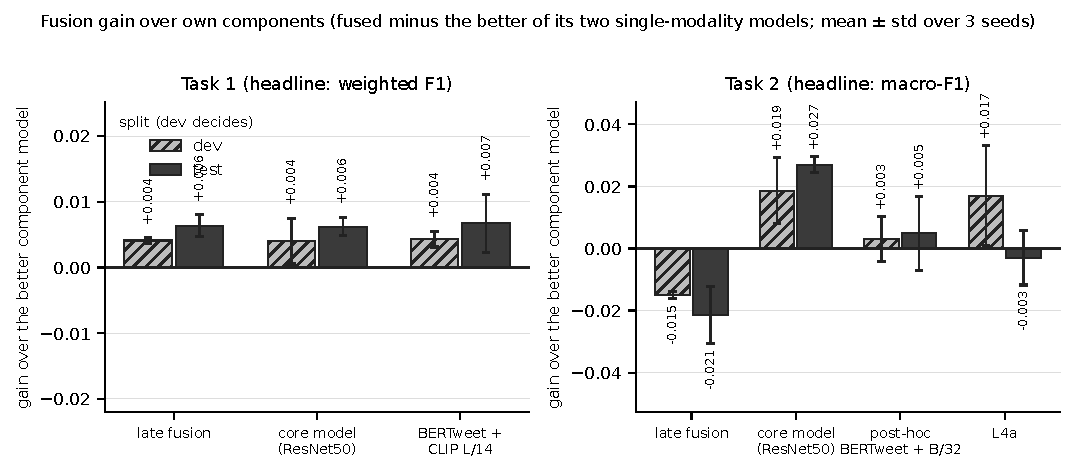
\includegraphics[width=0.92\textwidth]{figures/fig_c8_fusion_gain.pdf}
\caption{Fusion gain over own components (fused minus the better of its two single-modality models; development: hatched, test: solid; whiskers: s.d.\ over three seeds).}
\label{fig:fgain}
\end{figure*}

\textbf{Where each modality helps.} Fig.~\ref{fig:agree} splits both test sets by whether the text and image labels agree. In Task~1 (scored against the text label) the text model keeps its score on disagreed rows (weighted F1 0.80 against 0.86 on agreed rows) while the image head falls from 0.88 to 0.53; in Task~2 (scored against the image label) the image head keeps its score
(macro-F1 over the classes present 0.61 against 0.71) while the text model falls from 0.48 to 0.19. Fusion gains only where the labels agree, and loses where they disagree (Section~\ref{sec:discussion_modality}). These subset numbers are descriptive (no interval).

\begin{figure*}[t]
\centering
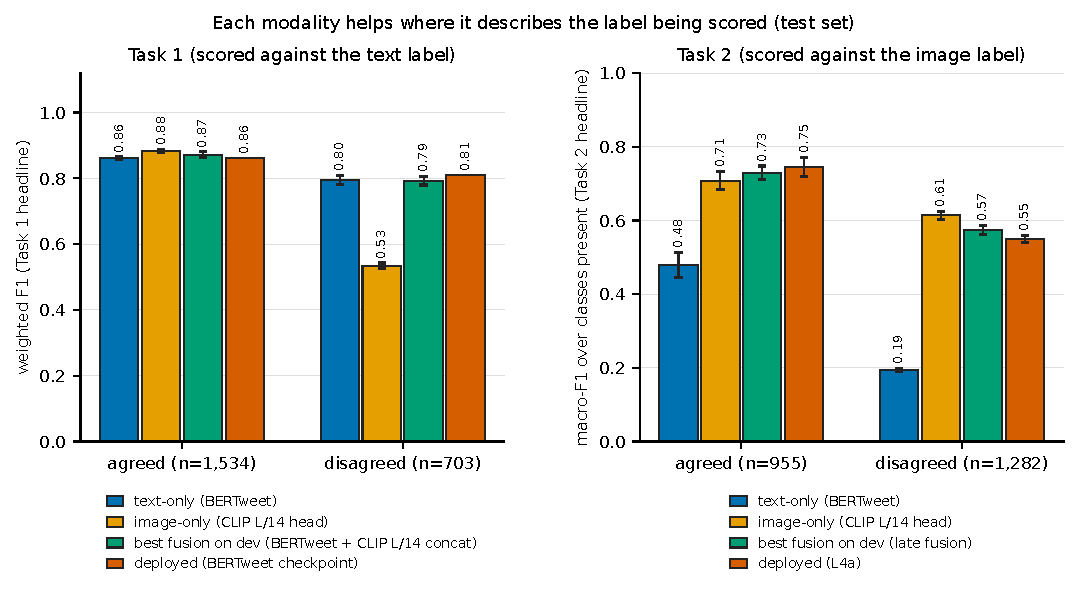
\includegraphics[width=0.92\textwidth]{figures/fig_c3_agreed_disagreed.pdf}
\caption{Each modality helps where it describes the label being scored (test set; bars: mean over three seeds, whiskers: s.d.; the deployed Task~1 model is a single checkpoint; Task~2 macro-F1 averages the classes present in the subset).}
\label{fig:agree}
\end{figure*}

\begin{figure}[t]
\centering
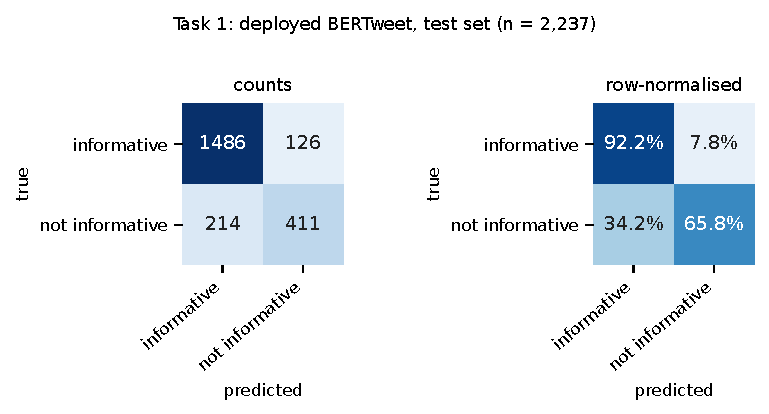
\includegraphics[width=0.95\columnwidth]{figures/fig_c1_t1_confusion.pdf}\\[2pt]
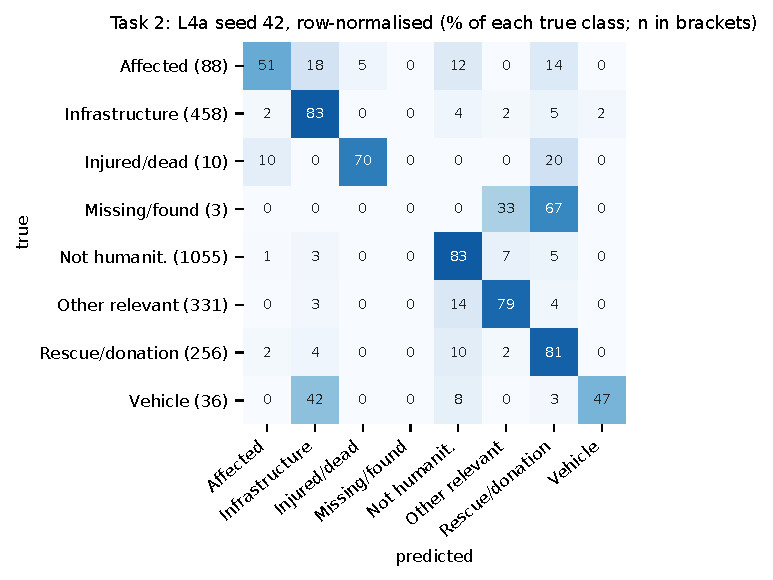
\includegraphics[width=0.85\columnwidth]{figures/fig_c2_t2_confusion.pdf}
\caption{Confusion matrices on the test set: Task~1 (deployed BERTweet; counts and row-normalised) and Task~2 (L4a seed 42; row-normalised, with the number of test rows per class).}
\label{fig:conf12}
\end{figure}

\textbf{Error analysis.} For the deployed models (Task~1 BERTweet, Task~2 L4a seed 42) we took 12 misclassified test examples per task by a rule fixed before looking at any example: the (true, predicted) pairs are ranked by their error count, and the first rows by index are taken from each pair in turn, at most three per pair (six for Task~1, which has only two pairs). Each error is assigned by written criteria to
\emph{text--image mismatch} (the text label differs from the image label), \emph{label ambiguity} (the predicted class is the true class's most-confused partner and the example is a near-duplicate of a training example with a conflicting label, or has at most five words), or \emph{model error}. Table~\ref{tab:errcounts} gives the counts over \emph{all} errors: 318 of the 440 Task~2 errors
(72\%) are rows on which the text and image labels disagree, against 134 of 340 for Task~1; the ambiguity criterion fires rarely (8 and 3 errors), so the sample, which follows the rank order of the confusion pairs, contains 2 and 0 of them.
Table~\ref{tab:errex} shows four examples per task; the contact sheets with the images are in the supplementary material.

\begin{table}[t]
\centering
\caption{Error analysis: category counts over \emph{all} test errors (rule-based categories, Section~\ref{sec:explore}) and in the 12-example sample per task.}
\label{tab:errcounts}
\footnotesize
\setlength{\tabcolsep}{3pt}
\begin{tabular}{llcccc}
\toprule
Task & Model & Errors & Mismatch & Ambiguity & Model error \\
\midrule
T1 & BERTweet (deployed) & 340 / 2,237 & 134 (5) & 8 (2) & 198 (5) \\
T2 & L4a seed 42 & 440 / 2,237 & 318 (6) & 3 (0) & 119 (6) \\
\bottomrule
\end{tabular}
\end{table}

\begin{table*}[t]
\centering
\caption{Examples of misclassified test tweets (the first four of the 12 per task, by the pre-set rule; all 24 are in the supplementary table and in the contact sheets). Confidence is the calibrated probability of the predicted class. Categories come from written criteria, not from reading each example.}
\label{tab:errex}
\scriptsize
\setlength{\tabcolsep}{3pt}
\begin{tabular}{llp{6.2cm}p{2.9cm}p{3.4cm}}
\toprule
\# & Category & Tweet (truncated) & True & Predicted ($p$) \\
\midrule
T1.1 & model error & Vet In Puerto Rico Hurricane Worse Than War - Shared from https://t.co/xpjHFigsHX. [htt... & not\_informative & informative (0.86) \\
T1.2 & text-image mismatch & Houston, Corpus Christi, Beaumont \& SE Texas seeing mosquitoes w/ Zika Virus: https://t... & not\_informative & informative (0.68) \\
T1.3 & label ambiguity & RT @RealDera: Hurricane Irma? Bring it bitch.???A https://t.co/4z6afuQdLZ & not\_informative & informative (0.85) \\
T1.4 & model error & \#Researchpreneur \#ScienceAlertsThe 2017 Hurricane Season Really Is More Intense Than???... & not\_informative & informative (0.79) \\
\midrule
T2.1 & model error & First Harvey, Then Irma and Jose. Why? It?s the Season. https://t.co/LWOrXWhFWN https:/... & Not humanitarian & Other relevant information (0.36) \\
T2.2 & model error & INBOX: @SpeakerStraus issues \#Harvey-related interim charges: \#txlege https://t.co/Y8t7... & Not humanitarian & Other relevant information (0.80) \\
T2.3 & model error & Tornado Watch for most of south Florida until 12AM Sept 10th https://t.co/jsC3W71b1h & Not humanitarian & Other relevant information (0.97) \\
T2.4 & model error & @realDonaldTrump And @fema ahead of \#HurricaneMaria and \#HurracaineIrma !! The \#FakeNew... & Not humanitarian & Rescue, volunteering or donation effort (0.59) \\
\bottomrule
\end{tabular}
\end{table*}

\textbf{Justification of the design choices.} Table~\ref{tab:justify} summarises, for each architectural choice, the alternatives tried, the development result, the verdict and the basis.

\begin{table*}[t]
\centering
\caption{Justification of each architectural choice: the choice, the alternatives tried, the result on the development split, the verdict and the basis (a resolvable difference, or the pre-registered tie-break to the simpler model). Exploratory comparisons; no multiplicity correction. Numbers are development-split values unless stated.}
\label{tab:justify}
\tiny
\setlength{\tabcolsep}{2.5pt}
\begin{tabular}{p{2.2cm}p{3.1cm}p{5.6cm}p{3.2cm}p{2.6cm}}
\toprule
Choice & Alternatives tried & Result & Verdict & Basis \\
\midrule
Task 1 text model: BERTweet (fine-tuned) & TF-IDF + LR, NB (unweighted / balanced / Complement), Random Forest, Linear SVM, BiLSTM + GloVe, majority class & dev weighted F1: BERTweet 0.8304, BiLSTM 0.8114, TF-IDF + LR 0.8109, NB (balanced) 0.7987, Random Forest 0.7983, Linear SVM 0.7940, majority 0.6036; BERTweet minus TF-IDF + LR +0.0195 [+0.0049, +0.0340]; BiLSTM minus TF-IDF + LR +0.0005 [-0.0129, +0.0133] & BERTweet better than TF-IDF + LR (CI excludes 0, positive at all 3 seeds); BiLSTM tied with TF-IDF + LR & pre-registered dev rule: resolvable \\
\midrule
Task 1 fusion: none (BERTweet text-only is deployed) & late fusion (calibrated), early fusion BERTweet + ResNet50 (guide's model), early fusion BERTweet + CLIP L/14 & dev weighted-F1 gain of the best fused model over BERTweet text-only +0.0043 [-0.0018, +0.0102]; guide's core model +0.0040 [-0.0014, +0.0095] & not distinguishable on dev (all three fused models tie); test intervals exclude 0 narrowly (reporting only); fusion helps only where text and image labels agree & tie-break (simplicity): the text-only model has the fewest components \\
\midrule
Task 1 loss: inverse-frequency weighted cross-entropy (kept) & unweighted cross-entropy (post-hoc arm) & dev balanced-accuracy gain of weighting +0.0175 [+0.0095, +0.0258]; not-informative recall 0.6704 vs 0.6043, informative recall 0.8950 vs 0.9262 & weighting changes the operating point (more not-informative predictions), it does not improve weighted F1 or macro-F1 detectably & kept because it was fixed by pre-registration; not a safety claim \\
\midrule
Task 2 text encoder (fine-tuned): DistilBERT in the deployed L4a & BERTweet (matched and 4-epoch recipes), TF-IDF + LR / SVM / ComplementNB, frozen MiniLM and MPNet heads (Section~\ref{sec:arch}) & dev macro-F1: BERTweet matched 0.3113, 4-epoch 0.3083, DistilBERT 0.2948, TF-IDF + LR 0.2700; BERTweet minus DistilBERT +0.0165 [-0.0004, +0.0334] & BERTweet consistent at every seed on dev but not resolvable (small, not robust); text-only models are far below image models & tie / not established: the deployed Task 2 model is unchanged (post-hoc comparison; raw vs cleaned input is a confound) \\
\midrule
Task 2 image backbone: CLIP (L/14 in the ablation-selected model, B/32 in the deployed one) & DINOv2, CLIP B/32, ResNet-50 (frozen features, image-only head; Section~\ref{sec:arch}) & dev macro-F1: CLIP L/14 0.6124, DINOv2 0.5758, CLIP B/32 0.5679, ResNet-50 0.5418; best minus DINOv2 +0.0366 [+0.0126, +0.0618], minus B/32 +0.0445 [+0.0111, +0.0797], minus ResNet-50 +0.0706 [+0.0372, +0.1084] & CLIP L/14 better than every alternative & pre-registered Day 2 rule (Section~\ref{sec:arch}, Table~\ref{tab:arch}): resolvable \\
\midrule
Task 2 fusion: the guide's core model (BERTweet + ResNet50) is not adopted; image-only / L4a remain & late fusion (calibrated), L4a cross-attention, concat, gated-late (Section~\ref{sec:arch}), the core model BERTweet + ResNet50 & core minus L4a, dev macro-F1 -0.0243 [-0.0579, +0.0064]; core minus image-only CLIP B/32 head -0.0074 [-0.0428, +0.0246]; trainable parameters 135,755,784 (core), 67,352,840 (L4a), 199,688 (image-only head) & tied on dev macro-F1 (dev weighted F1: worse, corroboration only); test macro-F1 worse for both (reporting only). Post-hoc, single factor changed: BERTweet + CLIP B/32 concat is not distinguishable from L4a (rows d4.t2b.posthoc\_clip\_b32\_vs\_L4a.*) and, against the core model, dev macro-F1 does not resolve it while dev weighted F1 and test are better (rows d4.t2b.posthoc\_clip\_b32\_vs\_core.*), which is consistent with the ResNet50 features, not BERTweet, being the weak part of the core model & tie-break (fewest trainable parameters): L4a over the core model; the image-only head over the core model \\
\midrule
Task 2 loss: inverse-frequency weighted cross-entropy (kept) & 9 alternatives (Section~\ref{sec:imbalance}): unweighted, sqrt-inverse, effective number, focal 1/2, focal 2 + inverse, sampler, logit adjustment, post-hoc & dev macro-F1 on L/14: focal loss (gamma 1) 0.6321, unweighted 0.6237, inverse-frequency 0.6124; on B/32: focal loss (gamma 2) 0.6016, inverse-frequency 0.5679; best minus inverse-frequency +0.0197 [-0.0122, +0.0480] (L/14), +0.0337 [-0.0019, +0.0651] (B/32) & 7 of 10 arms tied with the best on both backbones; the two backbones pick different arms & no new loss adopted (imbalance selection rule); inverse-frequency is 'not shown worse', not 'as good' \\
\midrule
Task 3: logistic probe predicts, 5-NN supplies the evidence & v2's 5-NN majority vote (k = 5), image-only and text-only retrieval (Section~\ref{sec:component}) & test macro-F1 0.6146 (hybrid probe) vs 0.4914 (5-NN); bootstrap +0.1231, 95\% interval +0.0615 to +0.1861 (test-sampling interval of Section~\ref{sec:component}; the probe's C was chosen on dev) & probe better than 5-NN & paired bootstrap on test (reporting, Section~\ref{sec:component}); not a dev-selected decision \\

\bottomrule
\end{tabular}
\end{table*}

\section{Discussion}

\textbf{The image carries the humanitarian task.} A 0.2M-parameter classifier on a frozen CLIP vector matches a 67M-parameter fusion model. This is a property of the task as labelled rather than a failure of fusion: the target is the image's annotation, so text can help only where the tweet describes the same thing as the image, and Table~\ref{tab:agree} shows that it does help there. Evaluating on text labels, or on the agreed subset as Ofli et al.\ did, would favour fusion. \todo{Partly contradicted by Task~1: on the full text-labelled Task~1, fusion is not distinguishable from text-only on development data (Section~\ref{sec:explore}); fusion gains appear on the agreed rows only. Rewrite.}

\textbf{Each modality helps where it describes the label being scored.}\label{sec:discussion_modality} The same pattern holds in both tasks (Fig.~\ref{fig:agree}). Task~1 is scored against the text label: fusion with image features gains weighted F1 on rows where the text and image labels agree and loses on rows where they disagree (late fusion: +0.041 against BERTweet on agreed rows, $-$0.061 on disagreed rows). Task~2 is scored against the image label and shows the mirror image: the text model collapses on disagreed rows, and fusion helps only on agreed rows. The subset results suggest that the label source, not the architecture, decides which modality carries the task; we did not train or score Task~2 on text labels or Task~1 on image labels, so this is an interpretation. \todo{Soften or cut: it rests on the descriptive agreed/disagreed split only.}

\textbf{Retrieval is better as evidence than as a vote.} Nearest-neighbour voting gives an intuitive explanation but a weaker prediction than a probe on the same features. Keeping the two roles separate preserves the explanation and adds a confidence signal: when the two disagree, both are close to guessing, and the tool asks a human to look.

\textbf{Data coverage matters more than refinements.} The largest single effect in the study is not an architectural change but the presence of two earthquake events, and it acts mostly through one rare class. For a deployed system, coverage of disaster types and of rare but critical categories matters more than model refinements, and several reasonable architectures cannot be told apart on test sets of this size.

\textbf{Label noise sets a ceiling.} Identical images with different severity labels show that the boundary between mild and severe damage is partly an annotator judgement, which limits the accuracy any Task~3 model can reach and helps explain why zero-shot models cannot recover it.

\textbf{Limitations.} \emph{Injured or dead people} (10 test rows) and \emph{missing or found people} (3) make macro-F1 unstable; the latter is never predicted correctly. All events are from 2017, and leave-one-disaster-out tests generalisation across these events only, with an image-only proxy for Task~2. The single-vector image stream reduces text-to-image attention to a projection. Three seeds resolve differences of about 0.01 at best, the Task~3 results and the classical Task~1 models are single deterministic runs, GPU training is not bit-for-bit repeatable (the deployed Task~1 checkpoint is a retrain of seed 42), the Task~1 leave-one-disaster-out column is a single seed, and about twenty further comparisons were made without multiplicity correction. The Task~1 and Task~2 splits overlap by tweet, which is safe only because no Task~1 model uses anything trained on Task~2 (asserted). The optional candidates of the guide's lists (DeBERTa-v3, ModernBERT, SigLIP, EfficientNet-B0, a zero-shot vision-language model, fine-tuning ResNet50 and a gated fusion for Task~1) were not run. Error-analysis categories are assigned by written criteria, not by human inspection.

\textbf{Responsible use.} The system is decision support, not an autonomous classifier. A missed report of injured or dead people is costly, and rare-class recall is the least reliable number in this report, so the output should never be used to deprioritise human review. Tweets are public but can contain personal information, and the tool shows retrieved past cases only from the training split.

% =====================================================================
\section{Conclusion and Future Work}

We presented a three-task triage pipeline for crisis tweets and evaluated it rigorously against our earlier version and against alternative designs, including the candidate models of our guide's lists: a fine-tuned BERTweet now serves Task~1, chosen by a rule fixed in advance, while the guide's early-fusion model did not beat our Task~2 model. Isolating each change showed that the earlier version's weaknesses came from data handling and leakage rather than from modelling, that the current design reaches equal Task~2 accuracy at a seventh of the compute, and that a hybrid of a trained probe and retrieved evidence improves Task~3 from 0.491 to 0.615 macro-F1 while flagging the cases a human should check. Ablations under rules fixed in advance show that the image carries the humanitarian task and that a larger CLIP encoder is the only design choice resolvable on these test sets.

Planned extensions are:
\begin{itemize}
\item \textbf{A larger image encoder in the fusion model}, since ViT-L/14 improves the image-only Task~2 model.
\item \textbf{A combined confidence score for Task~3} using both probe confidence and neighbour agreement, which are partly independent.
\item \textbf{Patch-token cross-attention for Task~2}, so that both attention directions operate over multiple elements.
\item \textbf{Agreed-label training and evaluation}, to compare directly with prior work.
\item \textbf{The optional candidates not run here}: DeBERTa-v3 or ModernBERT, SigLIP, a zero-shot vision-language model, fine-tuning ResNet50, and a gated fusion for Task~1. \todo{Decide which of the earlier items are now done and cut them.}
\item \textbf{More events and larger test sets for the rare classes}, and satellite imagery such as xBD~\cite{gupta2019} to complement ground-level images.
\end{itemize}

\section*{Acknowledgment}
Anurag V Rao (241IT011) and Chhitanshu Shekhar (241AI012) thank their project guide, Dr. Sowmya Kamath S, for her guidance and for the review that led to the comparison, class-imbalance and architecture studies.

% =====================================================================
\begin{thebibliography}{00}
\bibitem{alam2018} F. Alam, F. Ofli, and M. Imran, ``CrisisMMD: Multimodal Twitter datasets from natural disasters,'' in \textit{Proc. 12th Int. AAAI Conf. Web and Social Media (ICWSM)}, 2018, pp. 465--473.
\bibitem{ofli2020} F. Ofli, F. Alam, and M. Imran, ``Analysis of social media data using multimodal deep learning for disaster response,'' in \textit{Proc. 17th Int. Conf. Information Systems for Crisis Response and Management (ISCRAM)}, 2020.
\bibitem{imran2015} M. Imran, C. Castillo, F. Diaz, and S. Vieweg, ``Processing social media messages in mass emergency: A survey,'' \textit{ACM Computing Surveys}, vol. 47, no. 4, p. 67, 2015.
\bibitem{kapoor2023} S. Kapoor and A. Narayanan, ``Leakage and the reproducibility crisis in machine-learning-based science,'' \textit{Patterns}, vol. 4, no. 9, 2023.
\bibitem{radford2021} A. Radford \textit{et al.}, ``Learning transferable visual models from natural language supervision,'' in \textit{Proc. 38th Int. Conf. Machine Learning (ICML)}, 2021.
\bibitem{sanh2019} V. Sanh, L. Debut, J. Chaumond, and T. Wolf, ``DistilBERT, a distilled version of BERT: Smaller, faster, cheaper and lighter,'' arXiv:1910.01108, 2019.
\bibitem{reimers2019} N. Reimers and I. Gurevych, ``Sentence-BERT: Sentence embeddings using siamese BERT-networks,'' in \textit{Proc. EMNLP-IJCNLP}, 2019.
\bibitem{wang2020} W. Wang \textit{et al.}, ``MiniLM: Deep self-attention distillation for task-agnostic compression of pre-trained transformers,'' in \textit{Proc. NeurIPS}, 2020.
\bibitem{song2020} K. Song \textit{et al.}, ``MPNet: Masked and permuted pre-training for language understanding,'' in \textit{Proc. NeurIPS}, 2020.
\bibitem{oquab2024} M. Oquab \textit{et al.}, ``DINOv2: Learning robust visual features without supervision,'' \textit{Trans. Mach. Learn. Res.}, 2024.
\bibitem{he2016} K. He, X. Zhang, S. Ren, and J. Sun, ``Deep residual learning for image recognition,'' in \textit{Proc. IEEE Conf. Computer Vision and Pattern Recognition (CVPR)}, 2016.
\bibitem{vaswani2017} A. Vaswani \textit{et al.}, ``Attention is all you need,'' in \textit{Proc. NeurIPS}, 2017.
\bibitem{johnson2021} J. Johnson, M. Douze, and H. J\'egou, ``Billion-scale similarity search with GPUs,'' \textit{IEEE Trans. Big Data}, vol. 7, no. 3, pp. 535--547, 2021.
\bibitem{loshchilov2019} I. Loshchilov and F. Hutter, ``Decoupled weight decay regularization,'' in \textit{Proc. ICLR}, 2019.
\bibitem{lin2017} T.-Y. Lin, P. Goyal, R. Girshick, K. He, and P. Doll\'ar, ``Focal loss for dense object detection,'' in \textit{Proc. IEEE Int. Conf. Computer Vision (ICCV)}, 2017.
\bibitem{cui2019} Y. Cui, M. Jia, T.-Y. Lin, Y. Song, and S. Belongie, ``Class-balanced loss based on effective number of samples,'' in \textit{Proc. IEEE CVPR}, 2019.
\bibitem{menon2021} A. K. Menon \textit{et al.}, ``Long-tail learning via logit adjustment,'' in \textit{Proc. Int. Conf. Learning Representations (ICLR)}, 2021.
\bibitem{guo2017} C. Guo, G. Pleiss, Y. Sun, and K. Q. Weinberger, ``On calibration of modern neural networks,'' in \textit{Proc. 34th Int. Conf. Machine Learning (ICML)}, 2017.
\bibitem{efron1993} B. Efron and R. J. Tibshirani, \textit{An Introduction to the Bootstrap}. New York: Chapman \& Hall, 1993.
\bibitem{gupta2019} R. Gupta \textit{et al.}, ``Creating xBD: A dataset for assessing building damage from satellite imagery,'' in \textit{Proc. CVPR Workshops}, 2019.
\bibitem{nguyen2020} D. Q. Nguyen, T. Vu, and A. Tuan Nguyen, ``BERTweet: A pre-trained language model for English Tweets,'' in \textit{Proc. 2020 Conf. Empirical Methods in Natural Language Processing: System Demonstrations (EMNLP)}, 2020, pp. 9--14.
\bibitem{liu2019} Y. Liu \textit{et al.}, ``RoBERTa: A robustly optimized BERT pretraining approach,'' arXiv:1907.11692, 2019.
\bibitem{pennington2014} J. Pennington, R. Socher, and C. D. Manning, ``GloVe: Global vectors for word representation,'' in \textit{Proc. 2014 Conf. Empirical Methods in Natural Language Processing (EMNLP)}, 2014, pp. 1532--1543.
\bibitem{hochreiter1997} S. Hochreiter and J. Schmidhuber, ``Long short-term memory,'' \textit{Neural Computation}, vol. 9, no. 8, pp. 1735--1780, 1997.
\bibitem{schuster1997} M. Schuster and K. K. Paliwal, ``Bidirectional recurrent neural networks,'' \textit{IEEE Trans. Signal Processing}, vol. 45, no. 11, pp. 2673--2681, 1997.
\bibitem{breiman2001} L. Breiman, ``Random forests,'' \textit{Machine Learning}, vol. 45, no. 1, pp. 5--32, 2001.
\bibitem{pedregosa2011} F. Pedregosa \textit{et al.}, ``Scikit-learn: Machine learning in Python,'' \textit{J. Machine Learning Research}, vol. 12, pp. 2825--2830, 2011. % CHECK: start page 2825 confirmed on jmlr.org; end page from memory
\end{thebibliography}

\end{document}
